%Input preamble
%Style
\documentclass[12pt]{article}
\usepackage[top=1in, bottom=1in, left=1in, right=1in]{geometry}
\parindent 22pt
\usepackage{fancyhdr}

%Packages
\usepackage{adjustbox}
\usepackage{amsmath}
\usepackage{amsfonts}
\usepackage{amssymb}
\usepackage{bm}
\usepackage[table]{xcolor}
\usepackage{tabu}
\usepackage{color,soul}
\usepackage{makecell}
\usepackage{longtable}
\usepackage{multirow}
\usepackage[normalem]{ulem}
\usepackage{etoolbox}
\usepackage{graphicx}
\usepackage{tabularx}
\usepackage{ragged2e}
\usepackage{booktabs}
\usepackage{caption}
\usepackage{fixltx2e}
\usepackage[para, flushleft]{threeparttablex}
\usepackage[capposition=top,objectset=centering]{floatrow}
\usepackage{subcaption}
\usepackage{pdfpages}
\usepackage{pdflscape}
\usepackage{natbib}
\usepackage{bibunits}
\definecolor{maroon}{HTML}{990012}
\usepackage[colorlinks=true,linkcolor=maroon,citecolor=maroon,urlcolor=maroon,anchorcolor=maroon]{hyperref}
\usepackage{marvosym}
\usepackage{makeidx}
\usepackage{tikz}
\usetikzlibrary{shapes}
\usepackage{setspace}
\usepackage{enumerate}
\usepackage{rotating}
\usepackage{tocloft}
\usepackage{epstopdf}
\usepackage[titletoc]{appendix}
\usepackage{framed}
\usepackage{comment}
\usepackage{xr}
\usepackage{titlesec}
\usepackage{footnote}
\usepackage{longtable}
\newlength{\tablewidth}
\setlength{\tablewidth}{9.3in}
\setcounter{secnumdepth}{4}

\titleformat{\paragraph}
{\normalfont\normalsize\bfseries}{\theparagraph}{1em}{}
\titlespacing*{\paragraph}
{0pt}{3.25ex plus 1ex minus .2ex}{1.5ex plus .2ex}
\makeatletter
\pretocmd\start@align
{%
  \let\everycr\CT@everycr
  \CT@start
}{}{}
\apptocmd{\endalign}{\CT@end}{}{}
\makeatother
%Watermark
\usepackage[printwatermark]{xwatermark}
\usepackage{lipsum}
\definecolor{lightgray}{RGB}{220,220,220}
%\newwatermark[allpages,color=lightgray,angle=45,scale=3,xpos=0,ypos=0]{Preliminary Draft}

%Further subsection level
\usepackage{titlesec}
\setcounter{secnumdepth}{4}
\titleformat{\paragraph}
{\normalfont\normalsize\bfseries}{\theparagraph}{1em}{}
\titlespacing*{\paragraph}
{0pt}{3.25ex plus 1ex minus .2ex}{1.5ex plus .2ex}

\setcounter{secnumdepth}{5}
\titleformat{\subparagraph}
{\normalfont\normalsize\bfseries}{\thesubparagraph}{1em}{}
\titlespacing*{\subparagraph}
{0pt}{3.25ex plus 1ex minus .2ex}{1.5ex plus .2ex}

%Functions
\DeclareMathOperator{\cov}{Cov}
\DeclareMathOperator{\corr}{Corr}
\DeclareMathOperator{\var}{Var}
\DeclareMathOperator{\plim}{plim}
\DeclareMathOperator*{\argmin}{arg\,min}
\DeclareMathOperator*{\argmax}{arg\,max}

%Math Environments
\newtheorem{theorem}{Theorem}
\newtheorem{claim}{Claim}
\newtheorem{condition}{Condition}
\renewcommand\thecondition{C--\arabic{condition}}
\newtheorem{algorithm}{Algorithm}
\newtheorem{assumption}{Assumption}
\renewcommand\theassumption{A--\arabic{assumption}}
\newtheorem{remark}{Remark}
\renewcommand\theremark{R--\arabic{remark}}
\newtheorem{definition}[theorem]{Definition}
\newtheorem{hypothesis}[theorem]{Hypothesis}
\newtheorem{property}[theorem]{Property}
\newtheorem{example}[theorem]{Example}
\newtheorem{result}[theorem]{Result}
\newenvironment{proof}{\textbf{Proof:}}{$\bullet$}

%Commands
\newcommand\independent{\protect\mathpalette{\protect\independenT}{\perp}}
\def\independenT#1#2{\mathrel{\rlap{$#1#2$}\mkern2mu{#1#2}}}
\newcommand{\overbar}[1]{\mkern 1.5mu\overline{\mkern-1.5mu#1\mkern-1.5mu}\mkern 1.5mu}
\newcommand{\equald}{\ensuremath{\overset{d}{=}}}
\captionsetup[table]{skip=10pt}
%\makeindex

\setlength\parindent{20pt}
\setlength{\parskip}{0pt}

\newcolumntype{L}[1]{>{\raggedright\let\newline\\\arraybackslash\hspace{0pt}}m{#1}}
\newcolumntype{C}[1]{>{\centering\let\newline\\\arraybackslash\hspace{0pt}}m{#1}}
\newcolumntype{R}[1]{>{\raggedleft\let\newline\\\arraybackslash\hspace{0pt}}m{#1}}



%Logo
%\AddToShipoutPictureBG{%
%  \AtPageUpperLeft{\raisebox{-\height}{
\includegraphics[width=1.5cm]{uchicago.png}}}
%}

\newcolumntype{L}[1]{>{\raggedright\let\newline\\\arraybackslash\hspace{0pt}}m{#1}}
\newcolumntype{C}[1]{>{\centering\let\newline\\\arraybackslash\hspace{0pt}}m{#1}}
\newcolumntype{R}[1]{>{\raggedleft\let\newline\\\arraybackslash\hspace{0pt}}m{#1}}

\newcommand{\mr}{\multirow}
\newcommand{\mc}{\multicolumn}

%\newcommand{\comment}[1]{}

%Other parameters
\newcommand{\noutcomes}{95}
\newcommand{\noutcomesexpp}{357}
\newcommand{\noutcomesexpm}{343}
\newcommand{\noutcomesexpf}{355}
\newcommand{\treatsubsabc}{$75\%$}
\newcommand{\treatsubscarec}{$74\%$}
\newcommand{\treatsubscaref}{$63\%$}

%Counts
%Males
\newcommand{\positivem}{$78\%$}
\newcommand{\positivesm}{$29\%$}

%Females
\newcommand{\positivef}{$78\%$}
\newcommand{\positivesf}{$31\%$}

%Counts, control substitution
%Males
\newcommand{\positivecsnm}{$47\%$}
\newcommand{\positivescsnm}{$15\%$}

\newcommand{\positivecsam}{$79\%$}
\newcommand{\positivescsam}{$29\%$}

%Females
%% no alternative
\newcommand{\positivecsnf}{$84\%$}
\newcommand{\positivescsnf}{$55\%$}

%% alternative
\newcommand{\positivecsaf}{$79\%$}
\newcommand{\positivescsaf}{$33\%$}

%Pooled

%Effects
%Males

%Females
\newcommand{\empf}{$8$}
\newcommand{\yearsedf}{$1.7$}



%Pooled

%CBA
%IRR
%Males
\newcommand{\irrm}{$15\%$}
\newcommand{\irrsem}{$5\%$}

%Females
\newcommand{\irrf}{$9\%$}
\newcommand{\irrsef}{$7\%$}

%Pooled
\newcommand{\irrp}{$13\%$}
\newcommand{\irrsep}{$5\%$}

%BC
%Males
\newcommand{\bcm}{$11.24$}
\newcommand{\bcsem}{$4.60$}

%Females
\newcommand{\bcf}{$2.35$}
\newcommand{\bcsef}{$1.09$}

%Pooled
\newcommand{\bcp}{$5.63$}
\newcommand{\bcsep}{$2.15$}

%NPV streams
%Pooled
\newcommand{\parincomenpvp}{$\$119,346$}

\newcommand*\leftright[2]{%
  \leavevmode
  \rlap{#1}%
  \hspace{0.5\linewidth}%
  #2}

\newcommand{\orth}{\ensuremath{\perp\!\!\!\perp}}%
\newcommand{\indep}{\orth}%
\newcommand{\notorth}{\ensuremath{\perp\!\!\!\!\!\!\diagup\!\!\!\!\!\!\perp}}%
\newcommand{\notindep}{\notorth}

\externaldocument{abc_comprehensivecba_appendix-pub}
\externaldocument{abc_comprehensivecba_answerstoreferees}

\begin{document}

\begin{titlepage}
\newgeometry{top=.8in, bottom=.8in, left=.8in, right=.8in}

\title{\Large \textbf{Quantifying the Life-cycle \\ Benefits of an Influential Early Childhood Program}\thanks{This research was supported in part by grants from the Robert Wood Johnson Foundation's Policies for Action program, NICHD R37HD065072, the American Bar Foundation, the Buffett Early Childhood Fund, the Pritzker Children's Initiative, NICHD R01HD054702, NIA R01AG042390, and by the National Institute On Aging of the National Institutes of Health under Award Number P30AG024968. The views expressed in this paper are solely those of the authors and do not necessarily represent those of the funders or the official views of the National Institutes of Health. The authors wish to thank Frances Campbell, Craig and Sharon Ramey, Margaret Burchinal, Carrie Bynum, and the staff of the Frank Porter Graham Child Development Institute at the University of North Carolina Chapel Hill for the use of data and source materials from the Carolina Abecedarian Project and the Carolina Approach to Responsive Education. Years of partnership and collaboration have made this work possible. Collaboration with Andr\'{e}s Hojman, Yu Kyung Koh, Sylvi Kuperman, Stefano Mosso, Rodrigo Pinto, Joshua Shea, Jake Torcasso, and Anna Ziff on related work has strengthened the analysis in this paper. Collaboration with Bryan Tysinger of the Leonard D. Schaeffer Center for Health Policy and Economics at the University of Southern California on adapting the Future Adult Model is gratefully acknowledged. For helpful comments on various versions of the paper, we thank the editor, Harald Uhlig, two anonymous referees, St\'{e}phane Bonhomme, Fl\'{a}vio Cunha, Steven Durlauf, David Figlio, Dana Goldman, Ganesh Karapakula, Magne Mogstad, Sidharth Moktan, Tanya Rajan, Azeem Shaikh, Jeffrey Smith, Chris Taber, Matthew Tauzer, Ed Vytlacil, Jim Walker, Chris Walters, and Matt Wiswall. We benefited from helpful comments received at the Leonard D. Schaeffer Center for Health Policy and Economics in December, 2016, and at the University of Wisconsin, February, 2017. For information on the implementation of the Carolina Abecedarian Project and the Carolina Approach to Responsive Education and assistance in data acquisition, we thank Peg Burchinal, Carrie Bynum, Frances Campbell, and Elizabeth Gunn. For information on childcare in North Carolina, we thank Richard Clifford and Sue Russell. The set of codes to replicate the computations in this paper are posted in a repository. Interested parties can request to download all the files. The address of the repository is \url{https://github.com/jorgelgarcia/abccare-cba}. To replicate the results in this paper, contact any of the authors, who will put you in contact with the appropriate individuals to obtain access to restricted data. The Appendix for this paper is posted on \url{http://cehd.uchicago.edu/ABC_CARE}.}}

\author{
Jorge Luis Garc\'{i}a\\
Department of Economics\\
The University of Chicago \and
James J. Heckman \\
American Bar Foundation \\
Department of Economics\\
The University of Chicago \and
Duncan Ermini Leaf \\
Leonard D. Schaeffer Center \\  for Health Policy and Economics\\
University of Southern California \and
Mar\'{i}a Jos\'{e} Prados \\
Dornsife Center for \\ Economic and Social Research\\
University of Southern California}
\date{First Draft: January 5, 2016\\ This Draft: \today}

\maketitle
\thispagestyle{empty}
\restoregeometry
\end{titlepage}

\singlespacing
\thispagestyle{empty}
\begin{abstract}
\noindent This paper quantifies the life-cycle benefits of an influential high-quality early childhood program with outcomes measured through midlife. Guided by economic theory, we supplement experimental data with non-experimental data to forecast the life-cycle benefits and costs of the program. Our baseline estimate of the internal rate of return (benefit/cost ratio) is 13.7\% (7.3). We perform sensitivity analyses to our estimates of the empirical magnitudes of the numerous non-market benefits of the program. We account for model estimation and forecasting error. This paper is a template for synthesizing experimental and non-experimental data to estimate life cycle benefits of social programs. \textbf{[Word count: 100.]}
\end{abstract}

\noindent \textbf{Keywords}: Early childhood education, life-cycle benefits, long-term forecasts, program evaluation, rates of return. \\
\noindent \textbf{JEL codes}: J13, I28, C93\\


\bigskip
\begin{tabular}{ll}
Jorge Luis Garc\'{i}a                                          & James J. Heckman \\
Department of Economics                                 & Department of Economics \\
University of Chicago                                        & University of Chicago \\
1126 East 59th Street                                       & 1126 East 59th Street \\
Chicago, IL 60637                                             & Chicago, IL 60637 \\
Phone: 773-449-0744                                       & Phone: 773-702-0634  \\
Email: jorgelgarcia@uchicago.edu                    & Email: jjh@uchicago.edu \\
                                                                          & \\
Duncan Ermini Leaf                                           & Mar\'{i}a Jos\'{e} Prados \\
Leonard D. Schaeffer Center for                       & Dornsife Center for  \\
Health Policy \& Economics                              & Economic and Social Research \\
University of Southern California                       & University of Southern California \\
635 Downey Way                                              & 635 Downey Way        \\
Los Angeles, CA 90089                                    & Los Angeles, CA 90089 \\
Phone: 213-821-6474                                       & Phone: 213-821-7969 \\
Email: dleaf@healthpolicy.usc.edu                     & Email: prados@usc.edu \\

\end{tabular}

\clearpage

\restoregeometry
\doublespacing
\setcounter{page}{1}
%\pagenumbering{arabic}

\section{Introduction}

\noindent A large body of evidence documents that high-quality early childhood programs effectively promote the skills of disadvantaged children.\footnote{See \citet{Blau_Currie_2006_HEE}, \citet{Cunha_Heckman_ea_2006_HEE}, \citet{Duncan_Magnuson_2013_JEP}, \citet{Almond-Currie_2011_JEP}, and \citet{Elango_Hojman_etal_2016_Early-Edu} for surveys.} Much of this research estimates benefits in terms of cognitive test scores, school readiness, and measures of early-life social behavior. A few studies analyze longer-term benefits in completed education, adult health, crime, and labor income.\footnote{Examples include: \citet{Heckman_Moon_etal_2010_QE}, \citet{Havnes_Mogstad_2011_AEJEP}, and \citet{Campbell_Conti_etal_2014_EarlyChildhoodInvestments}.} Rigorous evidence on the long-term economic benefits of these programs is scarce.\footnote{\citet{Heckman_Moon_etal_2010_RateofReturn} present a life cycle cost-benefit analysis of the Perry Preschool Program. Our approach is more comprehensive in terms of outcomes analyzed and in providing a general methodology that can be replicated to assess the social efficiency of any other program.} Investment in high-quality early childhood education is only justified if social benefits exceed social costs.

This paper investigates the social efficiency of an influential pair of programs that target disadvantaged children. We analyze two virtually identical early childhood programs evaluated by randomized controlled trials with long-term follow up through the mid 30s conducted in North Carolina. They are the Carolina Abecedarian Project (ABC) and the Carolina Approach to Responsive Education (CARE)---henceforth ABC/CARE. Both programs were launched in the 1970s. The programs began early (at 8 weeks of life) and engaged participants until age 5. Participants experienced numerous positive treatment effects.\footnote{A companion paper, \citet{Garcia_Heckman_Ziff_2017_Gender-Diff_UNPUBLISHED}, documents these treatment effects.} Their parents (primarily mothers) received free childcare that enabled employment earnings and adult education. The program generated a $13.7\%$ per-annum tax-adjusted internal rate of return and a $7.3$ benefit/cost ratio.

The program is a prototype for many programs in place today.\footnote{Programs inspired by ABC/CARE have been (and are currently being) launched around the world. \citet{Sparling_2010_Highlights} and \citet{Ramey_Ramey_Lanzi_2014_Interventions} list numerous programs based on the ABC/CARE approach. The programs are: Infant Health and Development Program (IHDP) in eight different cities in the U.S. \citep{Spiker-etal_1997_Helping}; Early Head Start and Head Start. \citep{Schneider_McDonald-eds_2007_Scale-Up_Vol-1}; John's Hopkins Cerebral Palsy Study in the U.S. \citep{Sparling_2010_Highlights}; Classroom Literacy Interventions and Outcomes (CLIO) study. \citep{Sparling_2010_Highlights}; Massachusetts Family Child Care Study \citep{Collins_etal_2010_Massachusetts-Study}; Healthy Child Manitoba Evaluation \citep{Healthy_Child_Manitoba_2015_Starting-Early}; Abecedarian Approach within an Innovative Implementation Framework \citep{Jensen_Nielsen_2016_ABC-Programme-Pilot}; and Building a Bridge into Preschool in Remote Northern Territory Communities in Australia \citep{UMonash_Dataset_2015_URL}. Current Educare programs in the U.S. are also based on ABC/CARE \citep{Educare_2014_Research_Agenda,Yazejian_Bryant_2012_Educare}. Appendix~\ref{app:details-educare} lists these Educare programs, all of which implement curricula based on ABC/CARE.} About 19\% of all African-American children would be eligible for ABC/CARE today; 43\% of African-American children were eligible at its inception. Implementation of ABC/CARE on disadvantaged populations would be an effective, socially efficient strategy for promoting social mobility.\footnote{\citet{Garcia_2016_National-Implementation-ECI} report that if ABC/CARE were implemented on the current pool of eligible children in the population, the intra-black (black disadvantaged to black advantaged) gap in high-school graduation, years of education, employment and labor income at age 30 for females will be reduced by $110\%$, $76\%$, $22\%$, and $30\%$, respectively. It would eradicate the black--white high-school graduation gap, reduce the years of education gap to 0.12 years, reduce the employment gap to 14 percentage points, and reduce the labor income gap to 4,075 USD (2016). For males, the program would eradicate the intra-black high-school graduation gap, reduce the years of education gap to 0.18 years, reduce the employment gap to 9 percentage points, and reduce the labor income gap to 12,150 USD (2016).}

We confront a fundamental problem that arises in evaluating social programs. In our data, the oldest experimental subject is in his mid 30s. Yet we want to examine life-cycle returns. To do so, we supplement experimental data with non-experimental data on comparable older cohorts.

We forecast the life-cycle benefits and costs of the program using economic theory to guide construction of later life outcomes using non-experimental data.\footnote{\citet{Ridder_Moffitt_2007_hbk_metricsdata} provide a discussion of data combination methods. These methods are related to the older ``surrogate marker'' literature in biostatistics (see e.g.,\ \citealp{Prentice_1989_Surrogate_SiM}). However, as we note below, exogeneity is an integral part of the models we estimate, although it is not considered in the statistics literature. That literature does not provide testable predictions to validate the forecasts, which we produce using structural models.} We compute internal rates of return and benefit-cost ratios that encompass the large array of benefits and costs generated. We account for model estimation and forecasting error and the welfare cost of taxation required to fund the program. Our estimates are robust when subject to extensive sensitivity analyses.

This paper constructs a synthetic cohort from non-experimental samples that approximates the experimental sample in post-experimental years. Economic theory guides us in formulating and estimating invariant production functions that characterize program treatment effects. The estimated production functions depend on intermediate inputs changed by treatment that are measured in both experimental and non-experimental samples, but the production functions are not affected by treatment.\footnote{See \cite{Hurwicz_1962_structural} for the definition of policy invariance. We build on the methodology of \citet{Heckman_Pinto_etal_2013_PerryFactor}, who relate intermediate and long-term outcomes in a mediation analysis. They do not construct out of sample forecasts.} We test invariance of the production functions using non-experimental samples that overlap, in part, with the experimental sample. We can forecast experimental treatment effects using the estimated production functions applied to overlapping non-experimental data.

Our analysis is a template for estimating the life-cycle gains of social experiments for which there is less than full lifetime follow-up. Supplementing experimental data with non-experimental data using economic and econometric theory enhances the forecasting power of experiments. The quest for long-run answers from short-term experiments has recently led to informal procedures for estimating long-term benefits using short-term measures of childhood test scores \citep[e.g.][]{Kline_Walters_2016_QJE}. We show that these practices can be misleading.

The paper proceeds in the following way. Section~\ref{section:background} describes the ABC/CARE program. Section~\ref{section:cbamethodology} discusses our methodology for forecasting life-cycle outcomes and the evidence supporting our assumptions. Section~\ref{section:cbapractice} discusses how to implement our methodology. Section~\ref{section:cbaresults} reports baseline estimates of internal rates of return and benefit/cost ratios and an array of sensitivity analyses. Section~\ref{section:cbaresultscont} disaggregates the control group by computing presents social efficiency measures for the program relative to (a) alternative (low-quality) childcare options and (b) staying at home. All persons offered treatment accept. Section~\ref{section:bcaestimates} examines the predictive validity of widely used informal forecast methods for estimating the long-term benefits of programs with short-term follow up. Section~\ref{section:conclusion} summarizes our findings.

\section{ABC/CARE: Background} \label{section:background}

The Carolina Abecedarian Project and the Carolina Approach to Responsive Education (ABC/CARE) was an enriched childcare program that targeted the early years of disadvantaged, predominately African-American children in Chapel Hill, Durham, and Raleigh in North Carolina.\footnote{Both ABC and CARE were designed and implemented by researchers at the Frank Porter Graham Center of the University of North Carolina in Chapel Hill.} Appendix~\ref{appendix:background} describes the program in detail. We summarize its main features in the text.

The goal of these programs was to enhance the life skills of disadvantaged children. Both programs supported language, motor, and cognitive development as well as socio-emotional competencies considered crucial for school success including task orientation, the ability to communicate, independence, and pro-social behavior.\footnote{\citet{Sparling_1974_Synth_Edu_Infant_SPEECH, Ramey_Collier_etal_1976_CarolinaAbecedarianProject, Ramey_etal_1985_Project-CARE_TiECSE, Wasik_Ramey_etal_1990_CD, Ramey-etal_2012-ABC}.} The programs provided health screenings to treatment group members, but costs of health care were borne by parents.

ABC recruited four cohorts of children born between 1972 and 1976. CARE recruited two cohorts of children, born between 1978 and 1980. For both programs, families of potential participants were referred to researchers by local social service agencies and hospitals at the beginning of the mother's last trimester of pregnancy. Eligibility was determined by a score on a childhood risk index.\footnote{See  Appendix~\ref{app:eligibility-pop} for details on the construction of the index. It weights the following variables (listed from the most to the least important according to the index): maternal and paternal education, family income, father's presence at home, lack of maternal relatives in the area, siblings behind appropriate grade in school, family on welfare, father in unstable job, low maternal IQ, low siblings' IQ, social agency indicates that the family is disadvantaged, one or more family members has sought a form of professional help in the last three years, and any other special circumstance detected by program staff.}

The design and implementation of ABC and CARE were very similar. Both had two phases, the first of which lasts from birth until age 5. In this phase, children were randomly assigned to treatment. The second phase of the study consisted of child academic support through home visits from ages 5 through 8. The first phase of CARE, from birth until age 5, had an additional treatment arm of home visits designed to improve home environments.\footnote{\citet{Wasik_Ramey_etal_1990_CD}.} Our analysis uses the first phase and pools the ABC treatment group with of the CARE treatment groups. We do not use data from the CARE group that only received home visits in the early years. \cite{Campbell_Conti_etal_2014_EarlyChildhoodInvestments} test and do not reject the hypothesis that the CARE data through age 5 (without the home visits) and the ABC data (through age 5) come from the same distribution. 

In ABC, the initial sample consisted of 120 families. For reasons discussed in Appendix~\ref{appendix:background}, the study sample was reduced to 111 subjects: 53 in the treatment group and 58 in the control group. In CARE, the initial sample had 65 families: 23 were randomized to a control group, 25 to a family education treatment group, and 17 to a center-based childcare treatment group that followed ABC protocols. We present our (standard) methodology for assessing attrition and non-response in Appendix~\ref{app:method_partialobs} and apply it in our analysis.

The experiment collects annual observations on a variety of outcomes from ages 0 to 15. For both programs, data were annually collected on cognitive and socio-emotional skills, home environments, family structure, and family economic characteristics from birth until age 8. After age 8, data on cognitive and socio-emotional skills, education, and family economic characteristics were collected at ages 12, 15, 21, and 30.\footnote{At age 30, measures of cognitive skills are unavailable for both ABC and CARE.} In addition, there is information from administrative criminal records, a physician-administered medical survey, and a set of medical tests when the subjects were in their mid 30s.\footnote{See  Appendix~\ref{appendix:data} for a more comprehensive description of the data. There, we document the balance in observed baseline characteristics across the treatment and control groups after dropping the individuals for whom we have no crime or health information. There is substantial attrition for these data collections. The methodology that we propose addresses missing data in either of these two outcome categories.}

An important feature of the program is that many control-group children in both ABC and CARE attended alternative formal childcare arrangements (75\% and 74\% respectively). The alternative arrangements were generally lower quality than ABC/CARE.\footnote{See Appendix~\ref{appendix:tetanus} for details on these alternatives.} In our main analysis we compare treatment- and control-group children, irrespective of take-up of alternatives. In Section~\ref{section:cbaresultscont}, we disaggregate our analysis to distinguish treatment effects by control group. We now formalize our forecast procedure. 

\section{Forecasting Life-cycle Costs and Benefits: Method} \label{section:cbamethodology}

We now present our forecasting method in formal terms. For specificity, we focus on forecasting labor income, but our procedure is more general. We consider other outcomes in Section~\ref{section:cbapractice}.

$W=1$ indicates that parents referred to the program participate in the randomization protocol. $W=0$ indicates otherwise. $R$ indicates randomization into treatment ($R = 1$) or control ($R = 0$). $D$ indicates whether or not a family attends the program. $D = R$ implies compliance with the initial randomization protocol. Lower case variables $d$ and $r$ denote realizations of these random variables.

Individuals are eligible to participate in the program if their baseline background variables $\bm{B}\in\mathcal{B}_0$, where $\mathcal{B}_0$ is the set of scores on the risk index that determines program eligibility. Because all of the eligible people with the option to participate choose to do so $(W=1\text{, and } D=R)$, we can safely interpret the treatment effects generated by the experiment as average treatment effects for the population for the eligible population ($\bm{B}\in\mathcal{B}_0$) and not just mean treatment effects for the treated.\footnote{All providers of health care and social services (referral agencies) in the area of the ABC/CARE study were informed of the programs. They referred mothers whom they considered disadvantaged. Eligibility was corroborated before randomization. Our conversations with the program staff indicate that virtually all referred mothers attended and agreed to participate in the initial randomization \citep{Ramey-etal_2012-ABC}.}

Define $\bm{Y}^1_a$ as the outcome vector at age $a$ for the treated. $\bm{Y}^0_a$ is the age-$a$ outcome vector for the controls. At age $a$ the vector of average treatment effects for the population for which $\bm{B}\in\mathcal{B}_0$ is

\begin{equation}
\Delta_a  := \mathbb{E} \left[ \bm{Y}^1_a - \bm{Y}^0_a | W = 1 \right] = \mathbb{E} \left[\bm{Y}^1_a - \bm{Y}^0_{a} | \bm{B} \in \mathcal{B}_0 \right]. \label{eq:mainte}
\end{equation}

Randomization identifies this parameter in the experimental sample. A principal contribution of this paper is in providing a methodology for unbiased out of sample forecasts. We use a structural mediation model for treatment ($D=1$) and control ($D=0$) outcomes at age $a$ in sample $k \in \{e,n\}$, where $e$ denotes membership in the experimental sample and $n$ denotes membership in a non-experimental (auxiliary) sample. The functions for output $Y^d_{k,a}$ are:
\begin{eqnarray}
&Y^d_{k,a} = \phi^d_{k,a} (\bm{X}^d_{k,a}, \bm{B}_k) \ + \ \varepsilon^d_{k,a},  \label{eq:outcome} \\
 &d \in\{0,1\},  k\in\{e,n\}, \ \ a\in\{1,\dots,\bar{A}\} \nonumber
\end{eqnarray}
where $\phi^d_{k,a}\left( \cdot, \cdot \right)$ is a structural production relationship mapping inputs $\bm{X}^d_{k,a}, \bm{B}_k$ holding error term $\varepsilon^d_{k,a}$ fixed.\footnote{Fixing and conditioning are fundamentally different concepts. See \cite{Haavelmo_1943_Econometrica} and \citet{Heckman_Pinto_2015_EconometTheory} for discussions.} $ \bm{B}_k$ are baseline variables not affected by treatment. $\bm{X}^d_{k,a}$ are variables potentially affected by treatment. $\bar{A}$ is the oldest age considered in our analysis.

The relationship between inputs $\bm{X}^d_{k,a}, \bm{B}_k$ and outputs $Y^d_{k,a}$ can differ between experimental and non-experimental samples. The model characterizes the outcomes of the two treatment regimes in any sample, including the non-experimental sample, even though there are no empirical counterparts for those counterfactuals. Our analysis consists of providing conditions for identifying and estimating $\phi^d_{k,a}\left( \cdot, \cdot \right)$ in the non-experimental samples. The key condition is that there are differences in the technologies across treatment regimes given the production inputs: $\phi^d_{k,a} (\bm{X}^d_{k,a}, \bm{B}_k) = \phi_{k,a} (\bm{X}_{k,a}, \bm{B}_k)$ and $\varepsilon^d_{k,a} = \varepsilon_{k,a} d \in \{0,1\}$. \textbf{[Typist: George, it looks like he wants this to be equation 3, but I can't tell where the inline math ends and the equation begins]}. This condition is testable in the available experimental sample. Specifically, we adopt the following procedure for all outcomes:

\textbf{[JJH: Jorge, do we test equality of distributions of $\varepsilon^1_{k,a}$ and $\varepsilon^0_{k,a}$?]}

\begin{enumerate}
\item \textbf{Construct a Synthetic Cohort.} Select an eligible non-experimental sample ($\bm{B}_n \in \bm{B}_0$).
\item \textbf{Determine the Relevant Inputs.} Find a set of input variables $\bm{X}^d_{k,a}$ that (i) are available in the experimental and the non-experimental data; (ii) with support of the variables in the non-experimental data containing the support o their counterparts in the experimental data; (iii) that causally predict outcomes; and (iv) that are affected by treatment.
\item \textbf{Find Intermediate Inputs.} Find a set of input variables $\bm{X}^d_{k,a}$ that (i) are available in the experimental and the non-experimental data; (ii) the support of these variables in the non-experimental data contains the support in the experimental data; (iii) they are causal predictors of labor income; and (iv) they are affected by treatment.
\item \textbf{Estimate Equation~\ref{eq:outcome} and Test Condition~\ref{cond:cond3} in the Experimental Sample.}
\item Select Nonexperimental Counterparts to \ref{eq:outcome} using the outcome of Step 3, identify and estimate the technologies in Equation~\ref{eq:outcome} in the nonexperimental sample. A crucial step is establishing exogeneity of the inputs in the nonexperimental sample of accounting for nonexogeneity using appropriate econometric methods.
\item \textbf{Test the Validity of the Estimated Nonexperimental Model.} Using the nonexperimental model determined in Step 4, predict the within sample experimental treatment effects.
\item Forecast the experimental data out of sample using the model generated in Step 4 and validated in Step 5.
\item \textbf{Adjust for Forecast and Sampling Errors.} Construct standard errors that account for estimation and forecasting error in the experimental and the non-experimental datasets.
\end{enumerate}

For our labor income example, consider the forecasting of life-cycle labor income. In the non-experimental sample, we observe labor income from ages 21 to 67 (assumed to be age of retirement). We use these data to estimate a labor income function which depends on intermediate inputs (achievement test scores, education, and lagged labor income). These are the variables that are affected by treatment in the experimental data. Invariance of the labor income function across treatment regimes and across the experimental and non-experimental samples enhances the credibility of using the estimated equations to forecast post-experimental outcomes. In the experimental data, we observe labor income at ages 21 and 30. Within the experiment, we estimate the production function for labor income.We estimate and validate the production function in the non-experimental sample. Using the estimated technology, we forecast labor income through age 67. At age 30, we observe actual labor income, and can compare it with the forecast income using the technology estimated on non-experimental data. Forecasted and observed level of labor income at age 30 should be closely aligned under our invariance assumptions, and we find this to be true in our data. We elaborate on this procedure next.\footnote{Appendix~\ref{appendix:incomplete} provides more detail.}

\subsection{Constructing a Synthetic Cohort} \label{section:synthetic}

We use the Children of the National Longitudinal Survey of Youth (CNLSY) to construct synthetic cohorts from ages 21 to 29. We use both the National Longitudinal Survey of Youth 1979 (NLSY79) and the Panel Study of Income Dynamics (PSID) to forecast from ages 29 to 67. Whenever we use the NLSY79 and PSID together, we combine samples and use them as a joint sample. Thus, we use three non-experimental data sets to obtain information across our time span of interest, without placing specific weights in any particular sample. We satisfy support conditions.\footnote{See Appendix~\ref{app:containsupport}).}

We approximate $\bm{B}_{n} \in \mathcal{B}_0$ only and include observations satisfying the following criteria: 1. \textbf{NLSY79:} Black, labor income less than \$300,000 (2014 USD) in any given year; subjects born between 1957 and 1965; 2. \textbf{PSID:} Black; birth year between 1945 and 1981; and 3. \textbf{CNLSY:} Black, labor income less than \$300,000 (2014 USD) at any given year; subjects born between 1978 and 1983.

We then refine the samples further by constructing synthetic control and treatment groups using Mahalanobis' matching Algorithm~\ref{alg:match} in Appendix~\ref{appendix:methodology}. This algorithm provides a weight for each individual in the non-experimental sample according to her resemblance with individuals in the experimental sample. This is a straight matching procedure that does not necessarily impose exogeneity on the match variables. We use each of the following variables at all ages: year of birth, gender, and number of siblings at baseline. These variables are available across all non-experimental datasets. We construct one synthetic control group and one synthetic treatment group in each non-experimental sample (not one group for each age). In the experimental sample, all of the parents of children with characteristics $\bm{B}_{e} \in \mathcal{B}_0$ agree to participate in the program and satisfy these criteria. \textbf{[JJH: Jorge, this is a brand new procedure that ignores the discussion in the previous subsection]}

\textbf{[JJH: Section 3.1 is confusing. We go through this rigmarole to generate a sample for the model estimation? But the matching (not on our inputs) fits control group well - good enough. Does the matching fit treatment group well? If so, why do the rest - we can do Figure 1 with treatment group as well. Look - this is your work. I clearly do not understand it. You can have the whole bundle if you want. The logic of Section 3 is broken.]}

We can evaluate the validity of the synthetic control group \textbf{[JJH: Procedure for pooling? How do we get one group?]} by comparing average labor income of individuals in the non-experimental sample for whom $\bm{B}_{n} \in \mathcal{B}_0$ to average labor incomes of individuals in the synthetic control groups so constructed \textbf{[JJH: From the model is confusing. What model? Not equation 2.]}. They should coincide at each age. None of the non-experimental group received treatment. Further, they should coincide with observed control group labor income at age 30 in the experimental sample. Figure~\ref{figure:controltests} displays these tests. 

\begin{sidewaysfigure}[!htbp]
\centering
\caption{Labor Income Profile, Disadvantaged Individuals Synthetic Control Group Constructed by Matching in the Auxiliary Samples}\label{figure:controltests}
\begin{subfigure}[h]{0.5\textwidth}
		\centering
		\caption{Males}
		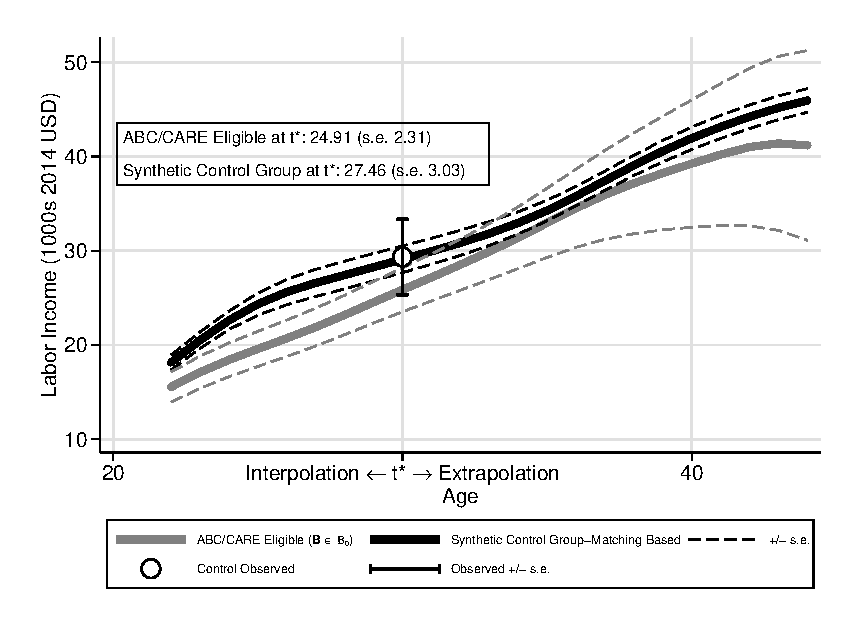
\includegraphics[width=\textwidth]{output/abccare_disad_1.eps}
\end{subfigure}%
\begin{subfigure}[h]{0.5\textwidth}
		\centering
		\caption{Females}
		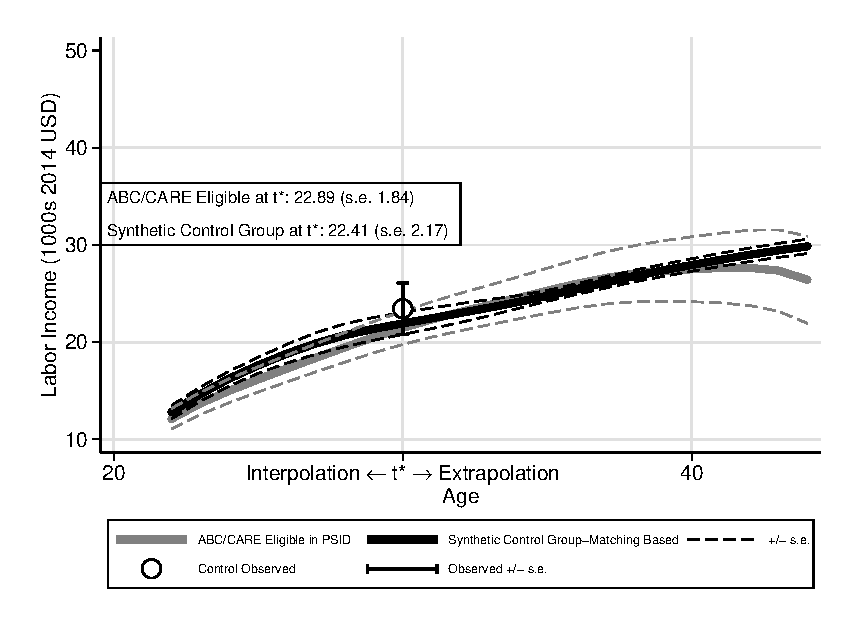
\includegraphics[width=\textwidth]{output/abccare_disad_0.eps}
\end{subfigure}
\footnotesize \justify
Note: Panel (a) displays the forecasted labor income for males in the auxiliary samples for whom $\bm{B} \in \mathcal{B}_0$, i.e., ABC/CARE eligible, and for the synthetic control group we construct based on the method proposed in this section. We combine data from the Panel Study of Income Dynamics (PSID), the National Longitudinal Survey of Youth 1979 (NLSY79), and the Children of the National Longitudinal Survey of Youth 1979 (CNLSY79). We highlight the observed labor income at oldest $a^*$ (age 30) for the ABC/CARE control-group participants. We stop at age 45 for want of data to compute the childhood risk index defining $\bm{B} \in \mathcal{B}_0$ in the auxiliary samples. \textbf{[JJH: Then how do we go out to age 67 as promised? This is very confusing]} Panel (b) displays the analogous figure for females. Standard errors are based on the empirical bootstrap distribution. $*$ is the oldest age in the experimental sample. 
\end{sidewaysfigure}

\subsection{Determining Intermediate Inputs} \label{section:inputs}

Intermediate inputs for labor income are: average PIAT achievement score from ages 5 to 7, completed education, labor income at age 21, and lagged labor income (which is forecasted after age 22). Table~\ref{table:predlaborincome} shows that these variables predict labor income and Appendix~\ref{app:containsupport} shows that there is common support across data sets. In the main text, we report treatment effects of the program on the intermediate inputs. This is critical for our forecasts, since we estimate an economic model in which the forecasted treatment effect are mediated by treatment effects on these variables. Table~\ref{table:summint} provides a summary.\footnote{We first present raw treatment-control mean differences. As we report in Table~\ref{table:summint}, the treatment effects are substantial across multiple outcomes. In some cases, this finding is at odds with what other studies report \citet{Ramey_etal_1985_Project-CARE_TiECSE,Clarke_Campbell_1998_ABC_Comparison_ECRQ,Campbell_Pungello_etal_2001_DP,Campbell_Ramey_etal_2002_ADS,Campbell_Wasik_etal_2008_ECRQ,Campbell_Conti_etal_2014_EarlyChildhoodInvestments}. The difference is explained, mainly, by the fact that we consider effects by gender.  Only \citet{Campbell_Conti_etal_2014_EarlyChildhoodInvestments} consider treatment effects by gender. They focus on health effects and find that men have many more positive effects especially in cardiovascular and metabolic conditions. This is consistent with the results we report below.}

\begin{table}[!htpb]
\begin{threeparttable}
\caption{Summary of Treatment Effects for Intermediate Inputs of Labor Income ($\bm{X}^d_{k,a}$)} \label{table:summint}
\centering
\begin{tabular}{lcccc}
\toprule
& \mc{2}{c}{Females} & \mc{2}{c}{Males} \\
\cmidrule(lr){2-3} \cmidrule(lr){4-5}
& Control & Average & Control & Average  \\
& Mean & Treatment Effect & Mean & Treatment Effect  \\
\midrule
Math Scores & $     95.82 $  & $      4.16 $ & $     95.04 $ & $      1.97 $ \\
\quad (ages 5-7)                    &                                               & ($      2.53 $) & & ($       2.44 $) \\
High School Graduation & $      0.51 $ & $      0.25 $ & $      0.61 $ & $      0.07 $ \\
\quad (age 30)                      &                                               & ($      0.12 $) & & ($      0.12 $) \\
College Graduation & $      0.08 $ & $      0.13 $ & $      0.12 $ & $      0.17 $ \\
\quad (age 30)                      &                                               & ($      0.09 $) & & ($      0.11 $) \\
Years of Education & $     11.76 $ & $      2.14 $ & $     12.90 $ & $      0.53 $ \\
\quad (age 30)                      &                                               & ($      0.62 $) & & ($      0.51 $) \\
Labor Income  & $ 10,847.45 $ & $  1,741.47 $ & $ 17,025.60 $ & $ -1,671.96 $ \\
\quad (age 21)                      &                                               & ($  2,429.99 $) & & ($  3,345.15 $) \\
Labor Income  & $ 23,443.42 $ & $  2,547.50 $ & $ 29,340.31 $ & $ 19,809.74 $ \\
\quad (age 30)                      &                                               & ($  5,833.99 $) & & ($ 14,795.66 $) \\
\bottomrule
\end{tabular}
% This file produced using scripts/abccare/cba/labor/income-inputs-description.do
\begin{tablenotes}
\footnotesize
\item Note: This table shows the control-group level and the raw mean difference between treatment and control (average treatment effects), by gender. PIAT scores have a sample mean of 100 and a standard deviation of 15. High school and college graduation are expressed in rates. Labor income is in 2016 USD. Average treatment effects are bolded when statistically significant at the 10\%.
\end{tablenotes}
\end{threeparttable}
\end{table}

Random assignment to treatment has statistically and economically significant effects on the intermediate inputs. For females, it increases the average PIAT score by almost a third of standard deviation (the test is standardized to an in-sample standard deviation of 15 units). For males, the effect is almost half of a standard deviation. The program substantially boosts high-school graduation for females and college graduation for both males and females. As a joint summary of these effects, we use years of education as an intermediate input. Labor income at age 21 is not greatly boosted by the program. This arises in part because treatment-group individuals are more likely to be enrolled in college at age 21 and thus not supply labor at this age. However, as the life-cycle evolves, lagged labor income is important for obtaining precise forecasts, as economic theory suggests. As the life cycle evolves, the program boosts annual labor income, especially for males, for whom the average treatment effect at age 30 is almost 20 thousand dollars.\footnote{Table~\ref{table:summint} displays age-21 and age-30 labor income because labor income is observed at ages 21 and 30 in the experimental sample. Labor income at age 30 is an input in our methodology only after age 30.}

\subsection{Identifying and Estimating $\phi^d_{k,a}\left( \cdot, \cdot \right)$ in the Non-experimental Sample}

\textbf{[JJH: Section 3.1 seems to say: we can approximate the control group with matching. It breaks the logic of the paper.]}

For identifying and estimating life-cycle treatment effects, forecasting the treatment-control mean difference suffices. This does not require us to take a position on the exogeneity of $\bm{X}^d_k, \: k \in \{e,n\}$ with respect to labor income. Simpler conditions, spelled out as Conditions~\ref{cond:cond1} and~\ref{cond:cond2} in Appendix~\ref{appendix:incomplete}, suffice. Exogeneity facilitates the use of economic theory to generate and interpret treatment effects, to test the validity of our synthetic control groups, and to find auxiliary sample counterparts to treatments and controls. It also facilitates a non-parametric approach that we discuss in Section~\ref{section:following}. Exogeneity also makes identification of $\phi^d_{k,a}\left( \cdot, \cdot \right)$ in the non-experimental sample straightforward. Assumption~\ref{ass:exog} spells out this assumption, which we initially make and then explore alternatives. \textbf{[JJH: We don't need this!] [JLG: Sure we don't and we said that in this very paragraph, but it gives us intuitive testable implications in levels as you wrote in the introduction.]}

\onehalfspacing
\begin{assumption}\label{ass:exog} \textbf{Exogeneity}
Let $\{ 1, \ldots, \bar{A} \}$ index the periods of a life cycle. For all $a, a'' \in \{ 1, \ldots, \bar{A} \}$ and for $d, d' \in \{0,1\}$,
\begin{equation}
\varepsilon^d_{k,a} \indep \bm{X}^{d^{\prime}}_{k,a^{''}} | \bm{B}_k = \bm{b}
\end{equation}
for all $\bm{b}$ in the support of $\bm{B}_k, \: k \in \{e,n\}$, where ``$\bm{M} \indep \bm{N}|\bm{Q}$'' denotes independence of $\bm{M}$ and $\bm{N}$ given $\bm{Q}$. $\square$
\end{assumption}
\doublespacing

To appreciate the benefit of Assumption~\ref{ass:exog}, consider the following example. Say we want to forecast labor income and we use years of education as a main component of $\bm{X}_{k,{a''}}^{d'}$. The joint distribution of $\varepsilon_{k,a}^d$ and $\bm{X}_{k,{a''}}^{d'}$ could differ substantially across experimental and non-experimental samples. In the experimental sample, years of education are boosted by treatment, which is randomly assigned. In the non-experimental samples, however, there is no experimental variation. Individuals with high observed levels of education could very well have high values of  $\varepsilon_{k,a}^d$ (e.g., ability bias). Assumption~\ref{ass:exog} avoids this problem when making forecasts.

We can test and relax this assumption. We report tests for endogeneity in the experimental and auxiliary samples used in this paper in Appendix~\ref{appendix:methodology}. To do so, we assume that $\varepsilon_{k,a}^d, k \in \{e,n\}$ follows a factor structure.\footnote{Factor structure models are widely used in structural estimation of production functions of skills during early childhood. See, e.g., \citet{Cunha_Heckman_2008_JHR} and \citet{Cunha_Heckman_etal_2010_est_tech_cognoncog}.} Once we condition on $\bm{X}_{k,a}^d$ and $\bm{B}_{k}$, we do not reject the null hypothesis of exogeneity. Below, we show that our results are robust to models that are more general than those in Equation~\eqref{eq:outcome} and, by construction, do not satisfy Assumption~\ref{ass:exog}. It turns out that in our samples the exogeneity requirement is satisfied.

We assume that the variables $\bm{X}_{k,a}^d$ fully summarize treatment in the sense that any effect that treatment has on outcomes operates through the inputs, $\bm{X}_{k,a}^d$, and not through shifts in the production function relating inputs to outputs (see \citealp{Heckman_Pinto_etal_2013_PerryFactor}). Assumption~\ref{ass:summary} formalizes this condition. \textbf{[JJH: Table 1 does not support our procedure.]}

\onehalfspacing
\begin{assumption} \label{ass:summary} \textbf{Structural Invariance}
For all $\bm{x}, \bm{b} \in supp(\bm{X}^d_{k,a}, \bm{B}_k), k \in \{e,n\}$
\begin{align}
\phi_{k,a}^0 \left( \bm{x}, \bm{b} \right) &= \phi_{k,a}^1 (\bm{x}, \bm{b}) \\   \nonumber                                                                     &=: \phi_{a} (\bm{x}, \bm{b}),
\end{align}
$\phi_{a}(\bm{x}, \bm{b})$ is the function generating the causal effect of setting $ \bm{B}_k=\bm{b}, \bm{X}^d_{k,a}=\bm{x}$ holding $\varepsilon^d_{k,a}$ fixed for $a \in \{1,\dots,A\}$. $\square$
\end{assumption}

\begin{remark} \textbf{Two Distinct Aspects of Structural Invariance}
Assumption~\ref{ass:summary} has two distinct aspects which could be broken down into two separate assumptions: (i) the structural relationships evaluated at the same arguments have identical values for treatment and control groups in the experimental sample, and (ii) the analogous holds across the experimental and non-experimental samples. 
\end{remark}

\begin{remark} \label{remark:cohort} \textbf{(No) Cohort Effects}
The second aspect of Assumption~\ref{ass:summary}, that the structural relationships are identical in the experimental and non-experimental samples, embeds a no cohorts effects assumption. That is: A structural function $\phi_{n,a}^d \left( \bm{x}, \bm{b} \right)$, which we identify and estimate in the non-experimental sample with subjects that are older than those in the experimental sample, is a valid means for forecast in the experimental sample. Note that this does not mean that there are not cohort effects in the outcome of interest, $Y_{k,a}^d$. Instead, it means that there are no cohort effects in the mapping between $\bm{X}_{k,a}, \bm{B}_k$ and $Y_{k,a}^d$. 
\end{remark}
\doublespacing

Assumption~\ref{ass:summary} combined with Assumption~\ref{ass:exog}, and normalizing $\mathbb{E}(\varepsilon^d_{k,a})=0$ for all $a \in \{1,\dots,A\}$, generates testable implications for our forecasting models. Exogeneity and invariance enable us to jointly test the two aspects of structural invariance, when $Y_{k,a}$ is observed in both the experimental and auxiliary samples:\footnote{The analogous implication if our only interest would be to forecast treatment effects is the following. Under our assumptions, experimental treatment effects should equal differences in the conditional means of the non-experimental samples evaluated at $\bm{X}_{n,a} = \bm{x}^1$ and  $\bm{X}_{n,a} = \bm{x}^0$:
\begin{eqnarray}
\mathbb{E} \left[ Y_{e,a}^1 |  \bm{X}_{e,a}^1 = \bm{x}^1, \bm{B}_e = \bm{b}, D = 1 \right] - \mathbb{E} \left[ Y_{e,a}^0 |  \bm{X}_{e,a}^0 = \bm{x}^0, \bm{B}_e = \bm{b}, D = 0 \right] = \nonumber \\
\mathbb{E} \left[ Y_{n,a} | \bm{X}_{n,a} = \bm{x}^1, \bm{B}_n = \bm{b} \right] - \mathbb{E} \left[ Y_{n,a} | \bm{X}_{n,a} = \bm{x}^0, \bm{B}_n = \bm{b} \right]. \label{eq:nec}
\end{eqnarray}

Note Equations~\eqref{eq:suff1} and~\eqref{eq:suff2} are sufficient conditions for Equation~\eqref{eq:nec} to hold.}

\begin{eqnarray}
\mathbb{E} \left[ Y_{e,a}^1 | \bm{X}_{e,a}^1 = \bm{x}, \bm{B}_{e} = \bm{b}, D = 1   \right] &=&  \mathbb{E} \left[ Y_{e,a}^0 | \bm{X}_{e,a}^0 = \bm{x}, \bm{B}_{e} = \bm{b}, D = 0   \right] \label{eq:suff1}  \\
\text{ and} & \nonumber \\
\mathbb{E} \left[ Y_{e,a}^d | \bm{X}_{e,a}^d = \bm{x}, \bm{B}_{e} = \bm{b}, D = d   \right] &=&  \mathbb{E} \left[ Y_{n,a} | \bm{X}_{n,a} = \bm{x}, \bm{B}_{n} = \bm{b} \right] \text{ for }  d \in \{0,1\}. \label{eq:suff2}
\end{eqnarray}

We briefly summarize tests for these implications here and present a discussion at length in Appendix~\ref{app:invariance}. We first use the experimental sample and ask if, once we account for the variables in $\bm{X}_{k,a}$, $R$ (randomization to treatment assignment in ABC/CARE, which, as discussed, is equivalent to $D$) predicts the outcome of interest, conditional on $\bm{B}_k$. This test verifies that $\bm{X}_{k,a}$ suffices to summarize the treatment generated by $R$. Under the null hypothesis, the coefficient associated with $R$ is zero. Failing to reject this is equivalent to failing to reject invariance across treatment regimes. Similarly, we can assess whether we fail to reject invariance across the samples by verifying that an indicator of sample membership (experimental or auxiliary) is not statistically different from zero when pooling the two samples.

Table~\ref{table:invariance} summarizes these tests. In Panel (a) we test invariance across treatment regimes using the experimental sample. We pool males and females to increase the power of our tests. We provide tests for both employment and labor income at age 30. The coefficient on $R$ is not significant when regressing either employment or labor income on mother's education (as a proxy for $\mathcal{B}_{0}$) and the intermediate inputs. For the case of employment, the test is precise. For the case of labor income, the test is less precise. After accounting for background variables and the intermediate inputs, average labor income is $284$ dollars (2014 USD) higher in the treatment group. This value is small if forced in the context that this is for annual labor income at age 30 and the average in the control group is $\$26,084$ (2014 USD).

In Panel (b) we display tests of invariance in labor income at age 30 across experimental and non-experimental samples. The tests are not as precise as in Panel (a), but, as before, the coefficients associated with the relevant indicator are relatively low if compared with the average of the variable (average labor income in the experimental and non-experimental sample for males and females are $\$40,007$ and $\$24,584$ \,and  $\$32,717$ and $24,098$ (2014 USD), respectively).

\begin{table}[!htpb]
\begin{threeparttable}
\caption{Intermediate Inputs of Labor Income, Summary of Treatment Effects} \label{table:invariance}
\centering
\begin{tabular}{lcccc} \toprule
 \multicolumn{5}{l}{\textbf{Panel (a). Invariance: Treatment Regimes}} \\
       & \multicolumn{2}{c}{Employment, age 30} &   \multicolumn{2}{c}{Labor Income, age 30} \\
       			      & coefficient & $p$-value & coefficient & $p$-value \\
$R$ &-0.008 & 0.550 & 283.356 & 0.490 \\
Mother's Education (at birth) & 0.031 & 0.150 & 496.581 & 0.430 \\
PIAT (5-7) & 0.031 & 0.150 & -81.009 & 0.595 \\
Years of Education (30) & 0.046 & 0.005 & 8,091.138 & 0.000 \\
Labor Income (21) & -0.000 & 0.850 & 0.130 & 0.330 \\ \\
$R^2$ & \multicolumn{2}{c}{0.279}  & \multicolumn{2}{c}{0.283}  \\
Observations & \multicolumn{2}{c}{380} & \multicolumn{2}{c}{310} \\ \\
$H_0$: model is null & \multicolumn{2}{c}{$F$ = 3.419} & \multicolumn{2}{c}{$F$ = 6.858} \\
& \multicolumn{2}{c}{$p$-value = 0.006} & \multicolumn{2}{c}{$p$-value = 0.000} \\ \midrule
 \multicolumn{5}{l}{\textbf{Panel (b). Invariance: Data Sources, Labor Income (Age 30)}} \\
       & \multicolumn{2}{c}{Females} &   \multicolumn{2}{c}{Males} \\
       			      & coefficient & $p$-value & coefficient & $p$-value \\
$K^*$ & 456.565 & 0.410  & 4,864.750 & 0.260 \\
Mother's Education (at birth) & -1,878.064 & 0.985  & 1,991.183 & 0.150 \\
PIAT (5-7) & 207.361 & 0.090 & 13.463 & 0.480 \\
Years of Education (30) & 3,381.137 & 0.000 & 11,855.479 & 0.000 \\
Labor Income (21) & 0.345 & 0.020 & 0.289 & 0.165 \\ \\
$R^2$ & \multicolumn{2}{c}{0.279}  & \multicolumn{2}{c}{0.283}  \\
Observations & \multicolumn{2}{c}{380} & \multicolumn{2}{c}{310} \\ \\
$H_0$: model is null & \multicolumn{2}{c}{$F$ = 28.945} & \multicolumn{2}{c}{$F$= 23.998} \\
& \multicolumn{2}{c}{$p$-value = 0.000} & \multicolumn{2}{c}{$p$-value = 0.000} \\ \bottomrule
\end{tabular}
\begin{tablenotes}
\footnotesize
\item * $K = 1$ if $k = e$; $K = 0$ if $k = m$\\
\item Note for Panel (a): Results from regressing, in the experimental sample, employment and labor income at age 30 on the variables listed in the left-most column. \\
\item Note for Panel (b): Results from regressing, in the pooled experimental and non-experimental  samples, labor income at age 30 on the variables listed in the left-most column by gender. 
\end{tablenotes}
\end{threeparttable}
\end{table}

\subsection{Following Steps} \label{section:following}

Invariance across treatment regimes and samples makes $\phi_{a} (\cdot, \cdot)$ the basic ingredient for forecasting in the experimental sample. Appendix~\ref{appendix:gmm} formalizes our estimation and data combination procedure in a GMM framework.\footnote{As both a referee and various commentators of our paper usefully pointed out, our identification and estimation strategies do not impose cross-sectional restrictions. This is a consequence of a data restriction: We use different datasets to identify and estimate the  $\phi_{a} \left( \bm{x}, \bm{b} \right)$ for each outcome (i.e., labor income, health, crime). Thus, the predictor variables that we are able to use differ across outcomes and we cannot perform this estimation. This implies an efficiency loss because it impedes us from imposing cross-sectional restrictions across outcomes.} By doing so, it provides a step-by-step estimation recipe. Figure~\ref{fig:labor-income-profiles} displays our forecasted labor income profiles. Forecasted and actual labor income are closely aligned, which is the final check for that we propose for our procedure.\footnote{The content in Figure~\ref{fig:labor-income-profiles} is sufficient but not necessary to calculate the gain of the program due to labor income. It would be sufficient to forecast the difference between the treatment and control groups. Forecasting the levels, however, provides us with additional testable implications. It also allow us to easily account for forecasting error and to verify that the life-cycle profiles that we estimate are comparable to observed profiles for similar socio-economic groups. The pattern of life-cycle labor income we generate is typical for that of low-skilled workers \citep{Blundell-etal_2015_J-Pub-E,Gladden_Taber_2000_WageProgression,Sanders-Taber_2012_AR,Lagakos_Moll_etal_2016_LifeCycle_NBER}.} We proceed similarly with the remaining outcomes---e.g.,\ parental labor income, crime, health. Computing the net present value, the internal rate of return and benefit/cost ratios are straightforward once the age-by-age forecasts are available.\footnote{Some practical details involved in doing this are in Appendices~\ref{app:method_irr} and \ref{app:method_cbratio}.} Finally, we perform inference using the  bootstrap. Our inference accounts for each step of our estimation procedure. A step-by-step recipe for our inference is in Appendix~\ref{appendix:bootstrap}.

\begin{sidewaysfigure}[!htbp]
\centering
\caption{Forecasted Labor Income Profiles for ABC/CARE Participants}\label{fig:labor-income-profiles}
\begin{subfigure}[h]{0.5\textwidth}
		\centering
		\caption{Males} \label{fig:labor-income-profilesc}
		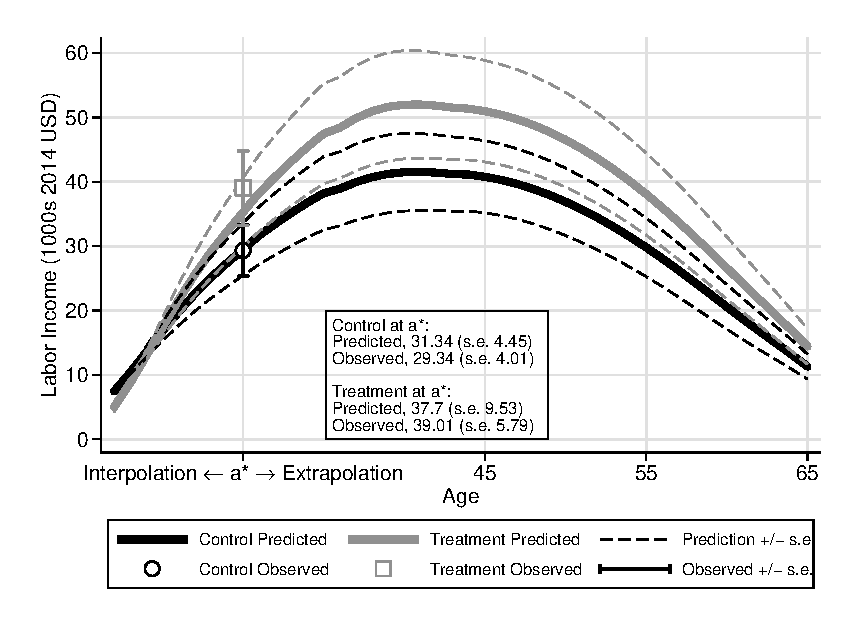
\includegraphics[width=\textwidth]{output/labor_25-65_pset1_mset1_male.eps}
\end{subfigure}%
\begin{subfigure}[h]{0.5\textwidth}
		\centering
		\caption{Females} \label{fig:labor-income-profilesa}
		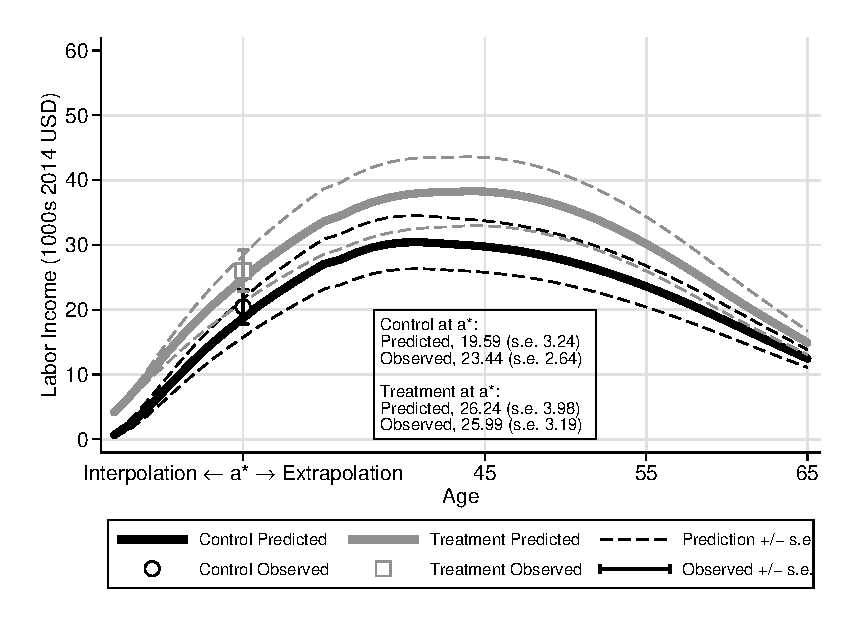
\includegraphics[width=\textwidth]{output/labor_25-65_pset1_mset1_female.eps}
\end{subfigure}
\footnotesize \justify
Note: Panel (a) displays the forecasted life-cycle labor income profiles for ABC/CARE males by treatment status, based on the method proposed in Section~\ref{section:cbamethodology}. We combine data from the Panel Study of Income Dynamics (PSID), the National Longitudinal Survey of Youth 1979 (NLSY79), and the Children of the National Longitudinal Survey of Youth 1979 (CNLSY79). We highlight the \textit{observed} labor income at $a^*$ (age 30) for the ABC/CARE control- and treatment-group participants. Panel (b) displays the analogous figure for females. Our forecasts go up to age 67, the age of assumed retirement. Standard errors are the respective standard deviations of the empirical bootstrap distribution. See  Appendix~\ref{appendix:methodology} for a discussion of our choice of predictors and a sensitivity analysis on those predictors. We under-predict labor income for both males and females. These differences, however, are not statistically significant (and labor income is a relatively minor component of the overall analysis for females).
\end{sidewaysfigure}

\subsection{Sensitivity and Alternative Approaches} \label{section:sens}

\begin{sidewaystable}[!htpb]
\resizebox{\columnwidth}{!}{%
\begin{threeparttable}
\caption{Net Present Value of Labor Income and Cost/Benefit Analysis Under Different Specifications for Labor Income Process}
\label{table:predsens}
\centering
\footnotesize
\begin{tabular}{L{2cm} *7{C{1.5cm}}} \toprule
& \multicolumn{3}{c}{ \textbf{Specification 1:}} & & \multicolumn{3}{c}{ \textbf{Specification 2:}}\\
& \multicolumn{3}{c}{Lagged component in $\bm{\phi}_{j,a}$} & & \multicolumn{3}{c}{No lagged component in $\bm{\phi}_{j,a}$} \\
& \multicolumn{3}{c}{ set $\bm{\rho} = 0$} & & \multicolumn{3}{c}{Unrestricted $\bm{\rho}$} \\[10pt]

& NPV & IRR & B/C & & NPV & IRR & B/C \\

\hline \\
Pooled & 71,345 & 0.13 & 6.29 & & 154,547 & 0.26 & 12.39 \\ 
& (86,343) & (.05) & (2.11) & & (187,036) & (0.11) & (5.16) \\ \\

Males & 300,896 & 0.13 & 11.1 & & 200,509 & 0.09 & 7.62 \\ 
& (241,588) & (0.06) & (6.35) & & (160,988) & (0.04) & (3.73) \\ \\ 

Females & 59,390 & 0.10 & 2.45 & & 79,441 & 0.15 & 3.61 \\ 
& (63,060) & (0.07) & (0.79) & & (99,416) & (0.11) & (1.56) \\ \\ \\

\midrule
& \multicolumn{3}{c}{ \textbf{Specification 3:}} & & \multicolumn{3}{c}{ \textbf{Specification 4:}}\\
& \multicolumn{3}{c}{Lagged component in $\bm{\phi}_{j,a}$} & & \multicolumn{3}{c}{Lagged component in $\bm{\phi}_{j,a}$; Permanent} \\
& \multicolumn{3}{c}{Unrestricted $\bm{\rho}$} & & \multicolumn{3}{c}{Transitory unobserved components} \\[10pt]

& NPV & IRR & B/C & & NPV & IRR & B/C \\

\hline \\
Pooled & 268,179 & 0.49 & 23.64 & & 46,953 & 0.09 & 4.14 \\ 
& (211,089) & (0.12) & (5.16) & & (25,323) & (0.01) & (0.62) \\ \\

Males &456,078 & 0.2 & 16.82 & & 74,775 & 0.03 & 2.76 \\ 
& (358,534) & (0.09) & (9.42) & & (54,752) & (0.01) & (1.44)  \\ \\ 

Females & 31,303 & 0.05 & 1.29 & & 19,959 & 0.03 & 0.82 \\ 
& (168,160) & (0.19) & (2.11) & & (34,142) & (0.04) & (0.43) \\ \\ \\


\midrule
& & & \multicolumn{3}{c}{\textbf{Specification 5:}} \\
& & & \multicolumn{3}{c}{ Fully Non-Parametric} \\[10pt]
& & & NPV & IRR & B/C \\
\hline \\
& & Pooled & 62,080 & 0.10 & 4.98 \\ 
& & & (75,030) & (0.03) & (2.07) \\ \\ 
& & Males & 289,471 & 0.13 & 11.01 \\ 
& & & (232,471) & (0.06) & (5.39) \\ \\ 
& & Females & 59,163 & 0.11 & 2.69 \\ 
& & & (74,039) & (0.08) & (1.16) \\ \bottomrule
\end{tabular}
\begin{tablenotes}
\normalsize
\item Note: This table displays the net present value of labor income in 2014 USD (treatment - control) using the five different specifications for forecasts that are explained below. Specification 1 is our baseline estimate. It also presents the calculation of the internal rate of return and the benefit/cost ratio of the program using these different net present values. Specification 1: forecast based on lagged outcome; no serial autocorrelation; and no fixed effect. Specification 2: forecast based on lagged outcome; arbitrary serial autocorrelation; and no fixed effect. Specification 3: forecast based on lagged outcome; first-order serial autocorrelation; and no fixed effects. Specification 4: forecast based on lagged outcome; no serial autocorrelation; and fixed effect. Specification 5: Forecast based on non-parametric matching in this section.\\
\item Model: With the exception of Specification 5, the different specifications are particular cases of the following model:

\begin{large}
\begin{eqnarray}
Y_{k,a}                   &=& \lambda_{0} + \lambda_{1} Y_{k,a-1} + \lambda_{2}  \bm{X}_{k,a} + \varepsilon_{k,a} \nonumber \\
\varepsilon_{k,a} &=& \underbrace{f}_{\text{Person-Specific Effect}} + \underbrace{\omega_{k,a}}_{\text{Possibly Serially Correlated Component}} \nonumber \\
\omega_{k,a}      &=& \rho \omega_{k,a-1} + \underbrace{U_{k,a}}_{\text{Independent Innovation}}.
\end{eqnarray}
\end{large}

\end{tablenotes}
\end{threeparttable}
}
\end{sidewaystable}

The forecasted present value of the gain induced by treatment using the model in Equation~\eqref{eq:outcome} pooling males and females is $636,674$ (s.e.\ $183,224$) in 2014 USD. We provide estimates of the present value gain when using more general labor income models (in which Assumption~\ref{ass:exog} does not hold) in Table~\ref{table:predsens}. When pooling males and females and when separating the samples by gender, the present value gains remain within a range that does not affect our estimated measures of overall efficiency.

A non-parametric forecasting alternative is to compress the whole procedure into the following. Under exogeneity assumption~\ref{ass:exog} and invariance condition~\ref{ass:summary} we can use matching to construct counterparts to the experimental treatment and control groups in the non-experimental sample.\footnote{\citet{Heckman_Ichimura_etal_1998_Econometrica} discuss this procedure.} Matching in this fashion creates direct counterparts in the auxiliary samples for each member of the experimental samples. Instead of estimating a model for the life-cycle profile of labor income, we directly use the matched counterparts' profiles. It is an intuitively appealing non-parametric estimator that is valid under exogeneity \citep{Heckman_Navarro_2004_REStat}. We discuss this approach in Appendix~\ref{appendix:match}. Matching is a non-parametric estimation procedure for conditional mean functions. There is close agreement between non-parametric estimates based on matching and more parametric model-based approaches in Table~\ref{table:predsens}.

\section{Forecasting Life-cycle Costs and Benefits: Practice} \label{section:cbapractice}

In this section, we adapt the methodology in Section~\ref{section:cbamethodology} to forecast the net benefit of the program due to parental income, crime, and health. The adaptation of our method has to do with practical rather than theoretical aspects involved in applying the methodology that we describe in Section~\ref{section:cbamethodology}. To illustrate this adaptation, we focus on health and provide brief details on crime and parental labor income. Appendices~\ref{appendix:crime} and~\ref{app:parentalincome} provide further documentation. Additional details for this are in Appendix~\ref{appendix:incomplete}. Straightforward calculations allow us to compute benefits and costs related to education and we describe those in Appendix~\ref{appendix:education}.

\subsection{Health}

We use health as an illustration because a major contribution of this paper forecasting and monetizing the life-cycle benefits of enhanced participant health using a version of Equation~\eqref{eq:outcome}, that includes a full vector of lagged dependent variables for different indicators of health status. This requires adapting the models of Section~\ref{section:cbamethodology}, as well as estimating a dynamic model of competing health risks \citep{Kalbfleisch_Prentice_1980_failure}. Three additional issues arise: (i) health outcomes such as diabetes or heart disease are absorbing states; (ii) chronic health outcomes are highly interdependent within and across time periods; and (iii) there is no obvious terminal time period for benefits and costs except death, which is endogenous.\footnote{For example, we extrapolate labor income until the retirement age of 67. For health, we need to forecast an age of death for each individual before extrapolating.}

Our auxiliary model for health is an adaptation of the Future Adult Model (FAM). This model forecasts health outcomes from the subjects' mid 30s up to their projected age of death \citep{Goldman_etal_2015_Future-Elderly-Model-Report}.\footnote{The simulation starts at the age in which we observe the subjects' age-30 follow-up.}  Appendix~\ref{appendix:health} discusses the FAM methodology in detail.

FAM passes a variety of specification tests and accurately forecasts health outcomes and health behaviors.\footnote{In Appendix~\ref{appendix:health-validation}, we present tests of the model's assumptions and predictive performance for population aggregate health and health behavior outcomes.} We initialize the health forecast model with the same variables used to forecast labor and transfer income, along with the initial health conditions as listed in Table~\ref{table:transition}.

Our methodology has five steps: (i) estimate age-by-age health state transition probabilities using the Panel Study of Income Dynamics (PSID); (ii) match these transition probabilities to the ABC/CARE subjects based on observed characteristics; (iii) estimate quality-adjusted life year (QALY) models using the Medical Expenditure Panel Survey (MEPS) and the PSID; (iv) estimate medical cost models using the MEPS and the Medicare Current Beneficiary Survey (MCBS), allowing estimates to differ by health state and observed characteristics; and (v) forecast the medical expenditures and QALYs that correspond to the simulated individual health trajectories.\footnote{As an intermediate step between (i) and (ii), we impute some of the variables used to initialize the FAM models (see  Appendix~\ref{section:FAM_ABC_impute}).}

Our microsimulation model starts with information on observed characteristics at age 30. Restricting it to the individuals for whom we have information from the mid 30s health survey allows us to account for components that are important for forecasting health outcomes. The models forecast the probability of being in any of the states in the horizontal axis of Table~\ref{table:transition} at age $a+1$ based on the state at age $a$, which is described by the vertical axis of the table.\footnote{In practice, the forecasts are based on two-year lags, due to data limitations in the auxiliary sources we use to simulate the FAM. For example, if the individual is 30 (31) years old in the age-30 interview, we simulate the trajectory of her health status at ages 30 (31), 32 (33), 34 (35), and so on until her projected death.} Absorbing states are an exception. For example, heart disease at age $a$ does not enter in the estimation of transitions for heart disease at age $a+1$ because it is an absorbing state: once a person has heart disease, she carries it through the rest of her life.

At each age, once we obtain the transition probability for each health outcome, we make a Monte-Carlo draw for each subject. Each simulation depends on each individual's health history and on her particular characteristics. For every simulated trajectory of health outcomes, we forecast the life-cycle medical expenditure using the models estimated from the MEPS and the MCBS. We then obtain an estimate of the expected life-cycle medical expenditure by taking the mean of each individual's simulated life-cycle medical expenditure.

\begin{figure}[!htbp]
\caption{Mean Quality-Adjusted Life Years: Forecasts and Comparison to PSID}\label{fig:qalys}
\centering
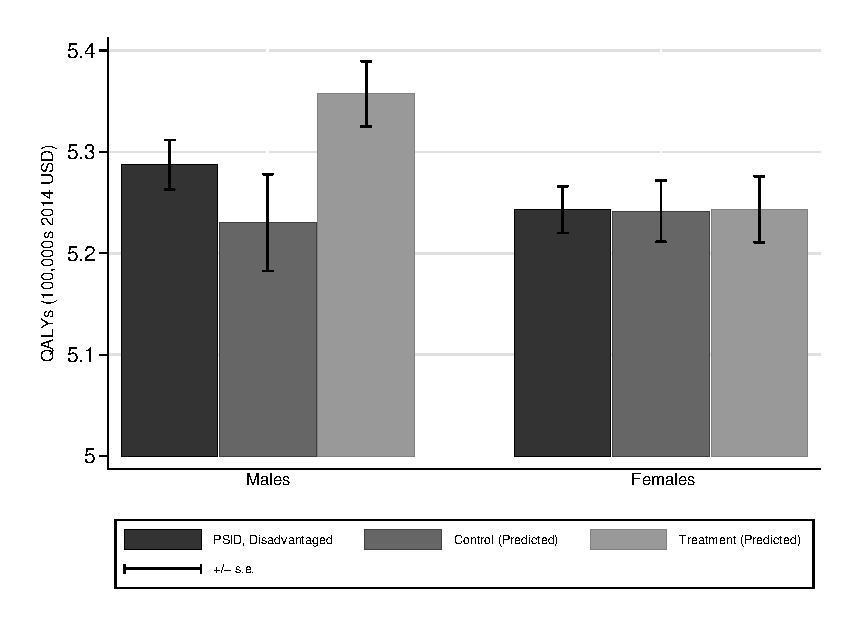
\includegraphics[width=.7\columnwidth]{output/qalyexppsid.eps}
\footnotesize \justify
Note:  This figure displays the life-cycle net present value of forecasted quality-adjusted life years (QALYs) for ABC/CARE males and females in the control group. The forecasts are based on combining data from the Panel Study of Income Dynamics (PSID), the Health Retirement Study (HRS), and the Medical Expenditure Panel Survey (MEPS). For each gender, we display a comparison to disadvantaged males and females in the PSID, where disadvantaged is defined as being African American and having at most 12 years of education. QALYs are the quality-adjusted life years accounting for the burden of disease. The black dots indicate that the bars are significantly greater than 0 at the 10\% level. This is calculated using the empirical bootstrap distribution.
\end{figure}

The models estimated using MCBS represent medical costs in the years 2007 to 2010. The MEPS estimation captures costs during 2008 to 2010. To account for real medical cost growth after 2010, we adjust each model's forecast using the method described in  Appendix~\ref{appendix:health-fam-simulation}.

The same procedure is applied to calculate QALYs. We compute a QALY model based on a widely-used health-related Quality-of-Life (HRQoL) measure (EQ-5D), available in MEPS.\footnote{A QALY is a measure which reweighs a year of life according to its quality given the burden of disease \citep{Dolan_1997_Modeling_MC,Shaw_etal_2005_EQ5D_MC}.} We then estimate this model using the PSID.

We estimate three models of medical spending: (i) Medicare spending (annual medical spending paid by parts A, B, and D of Medicare); (ii) private spending (medical spending paid by a private insurer or paid out-of-pocket by the individual); and (iii) all public spending other than Medicare. Each medical spending model includes the variables we use to forecast labor and transfer income, together with current health, risk factors, and functional status as explanatory variables.

We also calculate medical expenditures before age 30 (see Appendix~\ref{appendix:health-costs-before-age30}). The ABC/CARE interviews at ages 12, 15, 21 and 30 have information related to hospitalizations at different ages and number of births before age 30. We combine this information along with individual and family demographic variables to use MEPS to forecast medical spending for each age.

QALYs are crucial for our cost/benefit analysis because they monetize the health of an individual at each age. Figure~\ref{fig:qalys} plots our estimates of mean QALYs together with a PSID comparison for the control sample in an exercise analogous to that used to produce Figure~\ref{fig:labor-income-profiles}.\footnote{In our baseline estimation, we assume that each year of life is worth  $\$150,000$ (2014 USD). Our estimates are robust to substantial variation in this assumption, as we show in  Appendix~\ref{appendix:sensitivity}.} Although there is not a clear age-by-age treatment effect on QALYs, there is a statistically and substantively significant difference in the accumulated present value of the QALYs between the treatment and the control groups. The QALYs for female individuals in the control group match the QALYs of disadvantaged individuals in the PSID. For males, use of the PSID auxiliary sample to construct controls understates the net benefits of ABC/CARE.\footnote{In  Appendix~\ref{appendix:health} we further discuss and justify the parameterizations required to obtain estimates of QALYs. We only consider QALYs starting at age 30. \citet{Goldman_etal_2015_Future-America-Model} examine the sensitivity to these parameterizations and discuss alternative micro-simulations monetizing health condition.}

\subsection{Crime}

To estimate the life-cycle benefits and costs of ABC/CARE related to criminal activity, we use rich data on crime outcomes obtained from public records. Two previous studies consider the impacts of ABC on crime: \citet{Clarke_Campbell_1998_ABC_Comparison_ECRQ} use administrative crime records up to age 21, and find no statistically significant differences between the treatment and the control groups. \cite{Barnett_Masse_2002_benefitcost,Barnett_Masse_2007_EER} account for self-reported crime at age 21. They find weak effects based on self-reports, but they lack access to longer term, administrative data. The novelty of our study with respect to crime does not only consist of using administrative data allowing us to know the accumulated number of crimes that the children commit once they were in their mid 30s. It is also novel because we use micro-data specific to the state in which these individuals grew up, as well as other national datasets, to forecast criminal activity from the mid 30s to 50. See Appendix~\ref{appendix:crime} for a a complete discussion of our crime forecasts.

\subsection{Parental Labor Income} \label{section:pincome}

ABC/CARE offers childcare to the parents of treated children for more than nine hours a day for five years, 50 weeks a year. Only $27\%$ of participant mothers of children reported living with a partner at baseline and this status barely changed during the course of the experiment (see Appendix~\ref{appendix:background}). The childcare component generates substantial treatment effects on maternal labor force participation and parental labor income as reported. This arises from wage growth due to parental educational attainment and more work experience.\footnote{There is also an effect on maternal school enrollment. Some of the mothers decided to further enroll in school, obtained a higher degree, and that could be one of the reasons why they make more money afterward. We report these treatment effects in Appendix~\ref{appendix:background}. We quantify the cost of this additional education using the strategy in Appendix~\ref{appendix:education}.}

We observe parental labor income at eight different ages for the experimental subjects up through age 21.\footnote{The ages at which parental labor income is observed are 0, 1.5, 3.5, 4.5, 8, 12, 15, and 21. At age 21 the mothers of the ABC/CARE subjects were, on average, 41 years old.}$^,$\footnote{We linearly interpolate parental labor income for ages for which we do not have observations between 0 and 21.} An ideal approach would be to estimate the profile over the full life-cycle of mothers. We propose two different approaches for doing this in Appendix~\ref{app:parentalincome}: (i) an approach based on parameterizing parental labor income using standard Mincer equations; and (ii) an approach based on the analysis of Section~\ref{section:cbamethodology}. In Section~\ref{section:cbaresults}, we present estimates using the labor income through age 21 and using these two alternatives for projecting future labor income after age 21. The benefits of the program increase when considering the full life-cycles of mothers using either approach.

Any childcare inducements of the program likely benefit parents who, at baseline, did not have any other children ineligible for participation. If they did, then they might have had to take care of other children anyway, weakening the childcare-driven effect, especially if there are younger siblings present. In Appendix~\ref{app:parentalincome}, we show that the treatment effect for discounted parental labor income is much higher when the participant children have no siblings at baseline. The effect also weakens when comparing children who have siblings younger than 5 years old to children who have siblings 5 years old or older.\footnote{These patterns persist when splitting the ABC/CARE sample by gender, but the estimates are not precise because the samples become too small. See Appendix~\ref{app:parentalincome}.}

\subsection{Program Costs} \label{section:programscosts}

The yearly cost of the program was \$18,514 per participant in 2014 USD. We improve on previous cost estimates using primary-source documents.\footnote{Our calculations are based on progress reports written by the principal investigators and related documentation recovered in the archives of the research center where the program was implemented. We display these sources in Appendix~\ref{app:programcosts}. The main component is staff costs. Other costs arise from nutrition and services that the subjects receive when they were sick, diapers during the first 15 months of their lives, and transportation to the center. The control-group children also receive diapers during approximately 15 months, and iron-fortified formula. The costs are based on sources describing ABC treatment for $52$ children. We use the same costs estimates for CARE, for which there is less information available. The costs exclude any expenses related to research or policy analysis. A separate calculation by the implementers of the program indicates almost an identical amount (see  Appendix~\ref{app:programcosts}).} Appendix~\ref{app:programcosts} discusses the program costs in detail.

\section{Main Results and Sensitivity Analysis} \label{section:cbaresults}

Figure~\ref{figure:main} previews our findings. It displays the discounted (using a 3\% discount rate) life-cycle benefits and costs of the program (2014 USD) pooled across genders, over all categories, and for separate categories as well.\footnote{The baseline discount rate of 3\% is an arbitrary decision. Using discount rates of 0\%, 3\%, and 7\%, the estimates for the benefit/cost ratios are 17.40 (s.e.\ 5.90), 7.33 (s.e.\ 1.84), and 2.91 (s.e.\ 0.59), respectively. We report estimates for discount rates between 0\% and 15\% in  Appendix~\ref{appendix:varying-discount-rate}.} These benefits are the inputs of our baseline estimates for the per-annum internal rates of return and the benefit/cost ratio. We conduct extensive sensitivity and robustness analyses to produce ranges of plausible values for the estimates of the internal rate of return (8.0,\ 18.3) and the benefit/cost ratio (1.52,\ 17.40). The costs of the program are substantial, which has frequently been noted by critics.\footnote{See, e.g., \citet{Fox_News_2014_Head_Start_Effects} and \citet{Whitehurst_2014_Senate_Testimony}.} But so are the benefits, which far outweigh the costs. The individual gains in labor income, parental labor income, crime, and health are at least as large in magnitude as the costs. As a consequence, our measures of social efficiency remain statistically and economically significant even after eliminating the benefits from any one of the four main components that we monetize. No single component drives our results.

\begin{sidewaysfigure}[!htbp]
\caption{Net Present Value of Main Components of the Pooled (Over Gender) Cost/Benefit Analysis Over the Life Cycle per Program Participant, Treatment vs. Control}\label{figure:main}
\centering
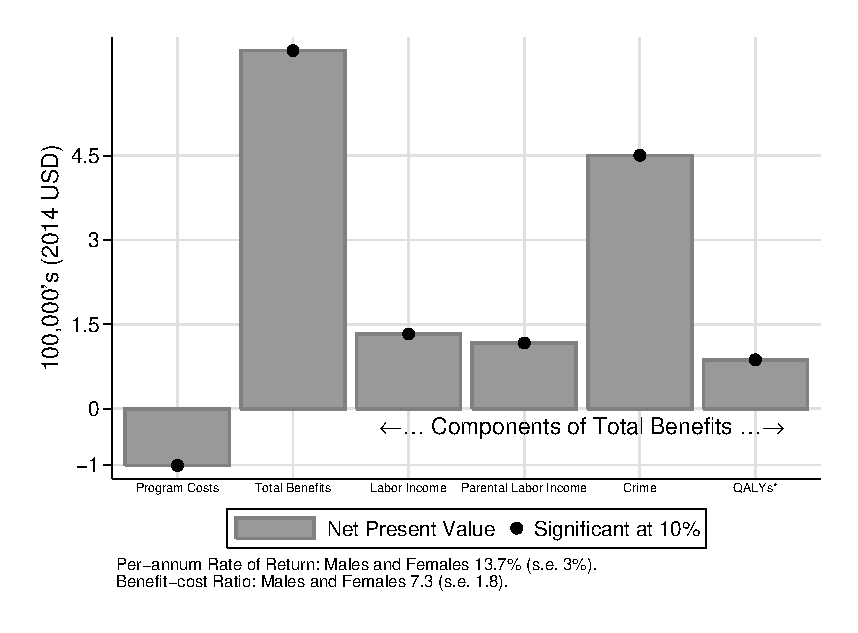
\includegraphics[width=.7\columnwidth]{output/abccare_npvssummredux.eps}
\footnotesize \justify
Note: This figure displays the life-cycle net present values per program participant of the main components of the cost/benefit analysis of ABC/CARE from birth to forecasted death, discounted to birth at a rate of 3\%. By ``net" we mean that each component represents the total value for the treatment group minus the total value for the control group. Program costs: the total cost of ABC/CARE, including the welfare cost of taxes to finance it. Total benefits: the benefits for \textit{all} of the components we consider. Labor income: total individual labor income from age 21 to the retirement of program participants (assumed to be at age 67). Parental labor income: total parental labor income of the parents of the participants from when the participants were ages 1.5 to 21. Crime: the total cost of crime (judicial and victimization costs). To simplify the display, the following components are not shown in the figure: (i) cost of alternative preschool paid by the control-group children's parents; (ii) the social welfare costs of transfer income from the government; (iii) disability benefits and social security claims; (iv) costs of increased individual and maternal education (including special education and grade retention); (v) total medical public and private costs. Inference is based on non-parametric, one-sided $p$-values from the empirical bootstrap distribution. We indicate point estimates significant at the $10\%$ level.
*QALYs refers to the quality-adjusted life years. Any gain corresponds to better health conditions until forecasted death, with $\$150,000$ (2014 USD) as the base value for a year of life.
\end{sidewaysfigure}


Table~\ref{table:bcsens} provides sensitivity analysis of the estimates to alternative assumptions. Table~\ref{table:irrsens} presents the corresponding internal rates of return. Pooling males and females, the results indicate that the program is socially efficient: the internal rate of return and the benefit/cost ratio are $13.7\%$ and $7.3$. \textit{Our baseline estimates indicate that the program generates a benefit of $7.3$ dollars for every dollar spent on it}. These estimates are statistically significant, even after accounting for sampling variation, serial correlation, and forecast error in the experimental and auxiliary samples and the tax costs of financing the program.\footnote{We obtain the reported standard errors by bootstrapping \emph{all} steps of our empirical procedure, including variable selection, imputation, model selection steps, and forecast error (see  Appendix~\ref{appendix:bootstrap}).} These benefits arise despite the fact that ABC/CARE was much more expensive than other early childhood education programs because the program used more services over a longer time period.

We accompany these estimates with an extensive set of sensitivity checks of statistical and economic interest. Our estimates are not driven by our methods for accounting for attrition and item non-response, by the conditioning variables, or by the functional forms of projection equations used when computing the net-present values.\footnote{See Appendix~\ref{appendix:methodology} for a detailed discussion.} Although the internal rate of return remains relatively high when using participant outcome measures only up to ages 21 or 30, the benefit/cost ratios indicate that accounting for benefits that go beyond age 30 is important. The return to each dollar is at most $3/1$ when only considering benefits up to age 30 (forecast span columns). Accounting for the treatment substitutes available to controls also matters. Males benefit the most from ABC/CARE relative to attending alternative childcare, while females benefit the most from ABC/CARE relative to staying at home. We explore this difference below.

\begin{sidewaystable}[!htpb]
\begin{threeparttable}
\caption{Sensitivity Analysis for Benefit/Cost Ratios}
\label{table:bcsens}
\centering
\scriptsize
\begin{tabular}{>{\bfseries}lcc|cc|cc} \toprule
	&	\multicolumn{2}{c}{\textbf{\textit{Pooled}}}	&	\multicolumn{2}{c}{\textbf{\textit{Males}}}	&	\multicolumn{2}{c}{\textbf{\textit{Females}}}	\\ 
Baseline	&	\multicolumn{2}{c}{5.69 (s.e. 2.32)}	&	\multicolumn{2}{c}{11.62 (s.e. 5.49)}	&	\multicolumn{2}{c}{2.60 (s.e. 0.98)}	\\ \\
\multicolumn{7}{l}{\textit{Baseline: IPW and Controls, Life-span up to Age 79, Treatment vs. Next Best, 50\% Marginal tax 50\% (deadweight loss), Discount rate 3\%, Parental}} \\	
\multicolumn{7}{l}{\textit{income 0 to 21 (child's age), Labor Income predicted from 21 to 65, All crimes (full costs), Value of life 150,000.}} \\ \\ \midrule	
Specification	&	\textit{No IPW}	&	\textit{and No Controls}	&	\textit{No IPW}	&	\textit{and No Controls}	&	\textit{No IPW}	&	\textit{and No Controls}	\\
	&	\textbf{6.17}	&	\textbf{5.35}	&	\textbf{11.94} 	&	\textbf{10.74}	&	\textbf{2.91}	&	\textbf{2.79}	\\
	&	(2.35)	&	(2.04)	&	(6.14)	&	(4.12)	&	(0.97)	&	(0.81)	\\ \midrule
Prediction	&	\textit{to Age 21}	&	\textit{to Age 30}	&	\textit{to Age 21}	&	\textit{to Age 30}	&	\textit{to Age 21}	&	\textit{to Age 30}	\\
Span	&	\textbf{1.55}	&	2.01	&	\textbf{2.17}	&	2.80	&	1.17	&	1.52	\\
	&	(0.39)	&	(0.88)	&	(0.74)	&	(1.96)	&	(0.43)	&	(0.48)	\\ \midrule
Counter-	&	\textit{vs. Stay at Home}	&	\textit{vs. Alt. Presch.}	&	\textit{vs. Stay at Home}	&	\textit{vs. Alt. Presch.}	&	\textit{vs. Stay at Home}	&	\textit{vs. Alt. Presch.}	\\
factuals	&	\textbf{4.44}	&	\textbf{6.58}	&	3.88	&	\textbf{10.85}	&	\textbf{4.89}	&	\textbf{2.40}	\\
	&	(1.68)	&	(2.22)	&	(2.78)	&	(4.14)	&	(1.50)	&	(0.94)	\\ \midrule
Deadweight-	&	\textit{0\%}	&	\textit{100\%\textit}	&	\textit{0\%}	&	\textit{100\%\textit}	&	\textit{0\%}	&	\textit{100\%\textit}	\\
loss	&	\textbf{8.50}	&	\textbf{4.29}	&	\textbf{17.43}	&	\textbf{8.71}	&	\textbf{3.69}	&	2.06	\\
	&	(3.47)	&	(1.75)	&	(8.19)	&	(4.14)	&	(1.43)	&	(0.79)	\\ \midrule
Discount 	&	\textit{0\%}	&	\textit{7\%}	&	\textit{0\%}	&	\textit{7\%}	&	\textit{0\%}	&	\textit{7\%}	\\
Rate	&	13.38	&	2.40	&	29.50	&	4.21	&	5.34	&	1.43	\\
	&	7.01	&	0.80	&	15.93	&	1.88	&	3.81	&	0.37	\\ \midrule
Parental	&	\textit{Mincer Life-cycle}	&	\textit{Life-cycle Prediction}	&	\textit{Mincer Life-cycle}	&	\textit{Life-cycle Prediction}	&	\textit{Mincer Life-cycle}	&	\textit{Life-cycle Prediction}	\\
Income	&	\textbf{5.92}	&	\textbf{5.60}	&	\textbf{11.80}	&	\textbf{12.36}	&	\textbf{2.88}	&	\textbf{3.27}	\\
	&	(2.32)	&	(2.39)	&	(5.49)	&	(5.68)	&	(1.02)	&	(1.21)	\\ \midrule
Labor	&	\textit{.5\% Annual Decay}	&	\textit{.5\% Annual Growth}	&	\textit{.5\% Annual Decay}	&	\textit{.5\% Annual Growth}	&	\textit{.5\% Annual Decay}	&	\textit{.5\% Annual Growth}	\\
Income	&	\textbf{5.48}	&	\textbf{5.90}	&	\textbf{10.76}	&	\textbf{12.49}	&	\textbf{2.47}	&	\textbf{2.74}	\\
	&	(2.25)	&	(2.41)	&	(5.33)	&	(5.71)	&	(0.87)	&	(1.10)	\\ \midrule
Crime	&	\textit{Drop Major Crimes}	&	\textit{Halve Costs}	&	\textit{Drop Major Crimes}	&	\textit{Halve Costs}	&	\textit{Drop Major Crimes}	&	\textit{Halve Costs}	\\
	&	\textbf{5.14} 	&	\textbf{4.07}	&	\textbf{11.82}	&	\textbf{8.33}	&	\textbf{2.72}	&	2.25	\\
	&	(2.30)	&	(1.50)	&	(5.59)	&	(3.64)	&	(1.04)	&	(0.95)	\\ \midrule
Health	&	\textit{Drop All}	&	\textit{Double Value of Life}	&	\textit{Drop All}	&	\textit{Double Value of Life}	&	\textit{Drop All}	&	\textit{Double Value of Life}	\\
(QALYs)	&	\textbf{4.85}	&	\textbf{6.56}	&	\textbf{10.61}	&	\textbf{12.63}	&	\textbf{2.48}	&	2.73	\\
	&	(2.32)	&	(2.54)	&	(5.37)	&	(5.90)	&	(0.97)	&	(1.26)	\\ \bottomrule
\end{tabular} 
\begin{tablenotes}
\scriptsize
\item Note: This table displays sensitivity analyses of our baseline benefit/cost ratio calculation to the perturbations indexed in the different rows. The characteristics of the \textit{baseline} calculation are in the table header. IPW: adjusts for attrition and item non-response (see  Appendix~\ref{app:method_partialobs} for details). Control variables: Apgar scores at ages 1 and 5 and a high-risk index (see  Appendix~\ref{appendix:results} for details on how we choose these controls). When forecasting up to ages 21 and 30, we consider all benefits and costs up to these ages, respectively. Counterfactuals: we consider treatment vs. next best (baseline), treatment vs. stay at home, and treatment vs. alternative preschools (see Section~\ref{section:cbaresultscont} for a discussion). Deadweight loss is the loss implied by any public expenditure (0\% is no loss and 100\% is one dollar loss per dollar spent). Discount rate: rate to discount benefits to child's age 0 (in all calculations). Parental labor income: see  Appendix~\ref{app:parentalincome} for details on the two alternative forecasts (Mincer and Life-cycle). Labor Income: 0.5\ annual growth (decay) is an annual wage growth (decay) due to cohort effects. Crime: major crimes are rape and murder; half costs takes half of victimization and judiciary costs. Health (QALYs): ``drop all'' sets the value of life equal to zero. Standard errors obtained from the empirical bootstrap distribution are in parentheses. Bolded $p$-values are significant at 10\% using one-sided tests. For details on the null hypothesis see Table~\ref{table:cba}.
\end{tablenotes}
\end{threeparttable}
\end{sidewaystable}

\begin{sidewaystable}[!htpb]
\begin{threeparttable}
\caption{Sensitivity Analysis for Internal Rate of Return}
\label{table:irrsens}
\centering
\scriptsize
% matrix: allirr file: allirr_sens.tex  25 Sep 2016 09:11:16
\begin{table}[htbp]
\begin{tabular}{lcccccc} \hline \hline
 & pooled  & pooled  & males  & males  & females  & females  \\  \hline 
baseline &     0.087 &     0.052 &     0.138 &     0.048 &     0.126 &     0.048 \\  
specification &     0.092 &     0.087 &     0.147 &     0.148 &     0.136 &     0.122 \\  
. &     0.059 &     0.032 &     0.060 &     0.037 &     0.044 &     0.039 \\  
predictiontime &     0.099 &     0.127 &     0.110 &     0.127 &     0.104 &     0.115 \\  
. &     0.056 &     0.051 &     0.047 &     0.051 &     0.045 &     0.043 \\  
counterfactual &     0.131 &     0.089 &     0.085 &     0.162 &     0.100 &     0.132 \\  
. &     0.046 &     0.057 &     0.038 &     0.044 &     0.034 &     0.039 \\  
dwl &     0.128 &     0.068 &     0.175 &     0.118 &     0.174 &     0.103 \\  
. &     0.089 &     0.037 &     0.063 &     0.042 &     0.064 &     0.037 \\  
parental &     0.104 &         . &     0.148 &         . &     0.142 &         . \\  
. &     0.069 &         . &     0.053 &         . &     0.053 &         . \\  
lincome &     0.080 &         . &     0.127 &         . &     0.122 &         . \\  
. &     0.053 &         . &     0.054 &         . &     0.047 &         . \\  
crime &     0.089 &     0.081 &     0.153 &     0.122 &     0.124 &     0.110 \\  
. &     0.052 &     0.051 &     0.043 &     0.046 &     0.044 &     0.044 \\  
health &     0.091 &     0.085 &     0.136 &     0.134 &     0.112 &     0.127 \\  
. &     0.053 &     0.052 &     0.049 &     0.053 &     0.058 &     0.045 \\  
\hline \hline \end{tabular}
\end{table}

\begin{tablenotes}
\scriptsize
\item Note: This table displays sensitivity analyses of our baseline internal rate of return calculation to the perturbations indexed in the different rows. The characteristics of the \textit{baseline} calculation are in the table header. IPW: adjusts for attrition and item non-response (see  Appendix~\ref{app:method_partialobs} for details). Control variables: Apgar scores at ages 1 and 5 and a high-risk index (see  Appendix~\ref{appendix:results} for details on how we choose these controls). When forecasting up to ages 21 and 30, we consider all benefits and costs up to these ages, respectively. Counterfactuals: we consider treatment vs. next best (baseline), treatment vs. stay at home, and treatment vs. alternative preschools (see Section~\ref{section:cbaresultscont} for a discussion). Deadweight loss is the loss implied by any public expenditure (0\% is no loss and 100\% is one dollar loss per dollar spent). Parental labor income: see  Appendix~\ref{app:parentalincome} for details on the two alternative forecasts (Mincer and Life-cycle). Labor Income: 0.5\ annual growth is an annual wage growth due to cohort effects; only benefit assumes labor income is the only benefit of the program. Crime: major crimes are rape and murder; half costs takes half of victimization and judiciary costs. Health (QALYs): ``drop all'' sets the value of life equal to zero. Bolded $p$-values are significant at 10\% using one-sided tests. For details on the null hypothesis see Table~\ref{table:cba}.
\end{tablenotes}
\end{threeparttable}
\end{sidewaystable}

Our baseline estimates account for the deadweight loss caused by distortionary taxes to fund programs, plus the direct costs associated with collecting taxes.\footnote{When the transaction between the government and an individual is a direct transfer, we consider 0.5 as the cost per each transacted dollar. We do not weight the final recipient of the transaction (e.g., transfer income). When the transaction is indirect, we classify it as government spending as a whole and consider its cost as 1.5 per dollar spent (e.g., public education).} We assume a marginal tax rate of $50\%$.\footnote{\citet{Feldstein_1999_REStat} reports that the deadweight loss caused by increasing existing tax rates (marginal deadweight loss) may exceed two dollars per dollar of revenue generated. We use a more conservative value (0.5 dollars per dollar of revenue generated). In Tables~\ref{table:bcsens}, \ref{table:irrsens}, and in  Appendix~\ref{appendix:varying-dwl}, we explore the robustness of this decision and find little sensitivity.} Our estimates are robust to dropping it to $0\%$ or doubling it to $100\%$ (deadweight loss columns). Our baseline estimate of benefit/cost ratios is based on a discount rate of $3\%$. Not discounting roughly doubles our benefit/cost ratios, while they remain statistically significant using a higher discount rate of $7\%$ (discount rate columns).

Parental labor income effects induced by the childcare subsidy are an important component of the benefit/cost ratio. We take a conservative approach in our baseline estimates and do not account for potential shifts in parental labor income profiles due to education and work experience subsidized by childcare (see the discussion in Section~\ref{section:pincome}). Our baseline estimates rely solely on parental labor income when participant children are ages 0 to 21. Alternative approaches considering the gain for the parents through age 67 generate an additional increase in the gain due to parental labor income (see parental labor income columns).

Individuals in ABC/CARE could experience positive cohort effects that might (i) make them more productive and therefore experience wage growth \citep{Lagakos_Moll_etal_2016_LifeCycle_NBER}; (ii) experience a negative shock such as an economic crisis and therefore experience a wage decline. Our estimates are robust when we vary annual growth and decay rates in labor income between $-0.5\%$ and $0.5\%$.

\begin{figure}[!htbp]
\caption{Benefit/Cost Ratio and Internal Rate of Return when Accounting for Different Combinations of the Main Benefits}\label{figure:vennpooled}
\centering
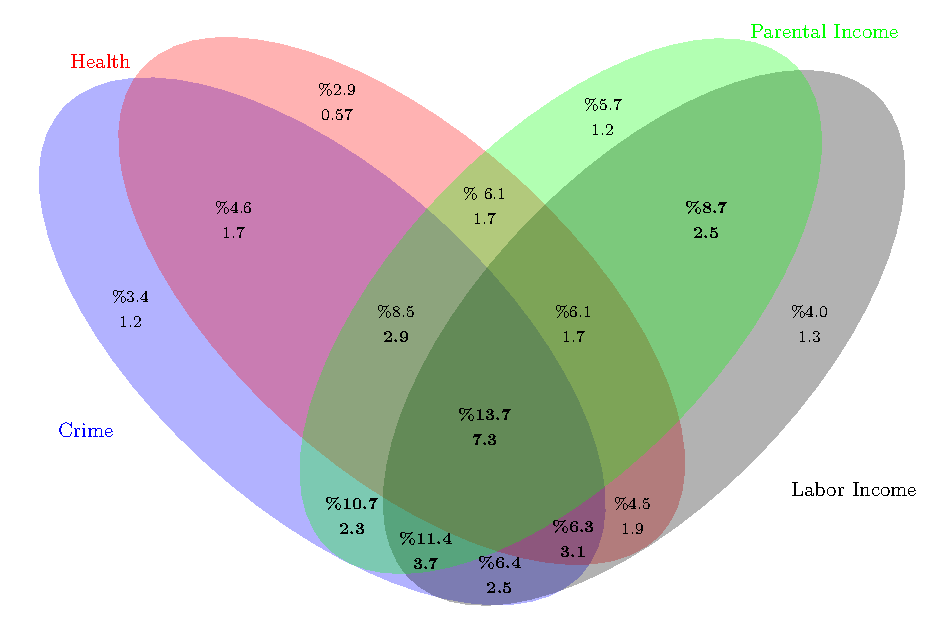
\includegraphics[width=.7\columnwidth]{output/venn_pooled.pdf}
\footnotesize \justify
Note: This figure presents all possible combinations of accounting for the benefits from the four major categories in our analysis. The non-overlapping areas present estimates accounting for a single category as the benefit. Where multiple categories overlap, we account for benefits from each of the overlapping categories. The other components remain constant across all calculations and are the same as in Figure~\ref{figure:main}. Health combines QALYs (quality-adjusted life years) and health expenditure. Inference is based on non-parametric, one-sided $p$-values from the empirical bootstrap distribution. We put boxes around point estimates that are statistically significant at the $10\%$ level.
\end{figure}

We also examine the sensitivity of our estimates to (i) dropping the most costly crimes such as murders and rapes;\footnote{Two individuals in the treatment group were convicted of rape and one individual in the control group was convicted of murder.} and (ii) halving the costs of victimization and judiciary costs related to crime. The first sensitivity check is important because we do not want our estimates to be based on a few exceptional crimes. The second is important because victimization costs are somewhat subjective (see  Appendix~\ref{appendix:crime-VI}). Our cost/benefit estimates are robust to these adjustments, even though crime is a major component of it. We also examine the sensitivity with respect to our main health component: quality-adjusted life years. This is an important component because healthier individuals survive longer, and treatment improves health conditions. It is important to note that this component largely accumulates later in life and therefore is heavily discounted. Dropping the component or doubling the value of life does not have a major impact on our calculations.

Figure~\ref{figure:vennpooled} summarizes the results from our extensive sensitivity analyses. It shows the estimated rates of return and benefit/cost ratios when we calculate our estimates under the assumption that only one of the many streams we consider is the source of the benefit. We calculate the estimates with all possible combinations of the main benefit and cost streams. Our measures of economic efficiency remain statistically and economically significant even after eliminating the benefits from any one of the four main components that we monetize. We report estimates from a variety of specifications of regressors and functional forms. Our estimates are robust to different plausible assumptions about the values of non-market outcomes, for which conventional estimates of standard errors are not available. Overall, our sensitivity analyses indicate that no single category of outcomes drives the social efficiency of the program. Rather, it is the life-cycle benefits across multiple dimensions of human development.

\section{Alternative and No Preschool} \label{section:cbaresultscont}

Our analysis so far compares the treatment to the control group, irrespective of the setting in which the control-group children developed. By construction, this exercise compares treatment to the ``next best'' alternative that the parents of the control-group children elected. As we document in Section~\ref{section:background}, almost 75\% of the control-group children were enrolled in an alternative. We refine our analysis to draw two further comparisons: (i) ABC/CARE compared to no treatment at all (so that the control child stayed at home); and (ii) ABC/CARE compared alternative preschool arrangements, which we describe in Section~\ref{section:background}.

All treatment-group children have the same exposure. We simplify the analysis of the controls by creating two categories. ``$H$'' indicates that the control-group child is in home care throughout the entire length of the program. ``$C$'' indicates that a control-group child is in alternative center childcare for any amount of time.\footnote{In our companion paper, \citet{Garcia_Heckman_Ziff_2017_Gender-Diff_UNPUBLISHED}, we show that this is a sensible assumption.} We thus compress a complex reality into two counterfactual outcome states at age $a$ for control-group subjects:
\begin{align*}
\bm{Y}_{a,H}^0 \quad &: \quad \textbf{ Subject received home care exclusively} \\
\bm{Y}_{a,C}^0 \quad &: \quad \textbf{ Subject received some alternative childcare}.
\end{align*}

We define $V$ as a dummy variable indicating participation by control-group children in an alternative childcare. $V=0$ denotes staying at home. The outcome when a child is in control status is
\begin{equation}
\bm{Y}^0_a : = \left( 1 - V \right) \bm{Y}^0_{a,H} + \left( V \right) \bm{Y}^0_{a,C}. \label{eq:meandiff}
\end{equation}

It is fruitful to assess the effectiveness of the program with respect to a counterfactual world in which the child stays at home full time. The associated causal parameter for those who would choose to keep the child at home is:
\begin{equation}\label{eq:influenza}
\bm{\Delta}_a \left(V = 0 \right) :=   \mathbb{E} \left[ \bm{Y}^1_a - \bm{Y}^0_a | V = 0, W = 1 \right] = \mathbb{E} \left[\bm{Y}^1_{a} - \bm{Y}^0_{a,H} | V = 0, \bm{B} \in \mathcal{B}_0 \right].
\end{equation}

It is also useful to assess the average effectiveness of a program relative to attendance in an alternative childcare center for those who would choose an alternative:

\begin{equation}\label{eq:smallpox}
\bm{\Delta}_a \left( V =1 \right) :=   \mathbb{E} \left[ \bm{Y}^1_a - \bm{Y}^0_a | V = 1, W = 1 \right] = \mathbb{E} \left[\bm{Y}^1_a - \bm{Y}^0_{a,C} | V = 1, \bm{B} \in \mathcal{B}_0 \right].
\end{equation}

Random assignment to treatment does not directly identify \eqref{eq:influenza} or \eqref{eq:smallpox}. Econometric methods are required to identify these parameters. The estimates that we provide in this paper rely on matching (conditioning on observables) to control for selection into the home or take-up of alternatives. In \citet{Garcia_Heckman_Ziff_2017_Gender-Diff_UNPUBLISHED}, we document that alternative strategies provide similar results. We combine the matching strategies with the methodology in Section~\ref{section:cbamethodology} to produce forecasts and provide measures of social efficiency refining the counterfactual comparison for the control-group children.

Figure~\ref{fig:npvsgender} summarizes the results from this exercise. There are substantial differences between males and females in one counterfactual: treatment vs. alternative preschools. The estimated treatment effects are very similar across genders for treatment compared to those staying at home full time. Males benefit much more from treatment relative to alternative preschools compared to their benefits from treatment relative to staying at home. This result is consistent with findings noted elsewhere: (i) stark gender differences resulting from attending low-quality childcare; and (ii) females are less sensitive to uncertain environments. We thoroughly discuss the mechanisms underlying these gendered effects and their consistency with the literature in \citet{Garcia_Heckman_Ziff_2017_Gender-Diff_UNPUBLISHED}, and focus this discussion on criminal outcomes in \citet{Garcia_etal_2019_ECE_IMHJ}.

Our evidence does not indicate that the program has no benefits for females. When compared to staying at home, there is a gain of 4.93 dollars per dollar invested. When we decompose the net-present value for each of the components that we monetize, we find substantial benefits for females across a variety of categories, including health and crime. For males, the magnitudes are noticeably increased when comparing outcomes from treatment to outcomes from attending alternative preschools.

\begin{sidewaysfigure}[!htbp]
\centering
\caption{Life-cycle Net Present Value of Main Components of the CBA}\label{fig:npvsgender}
\begin{subfigure}[h]{0.5\textwidth}
		\centering
		\caption{Males}
		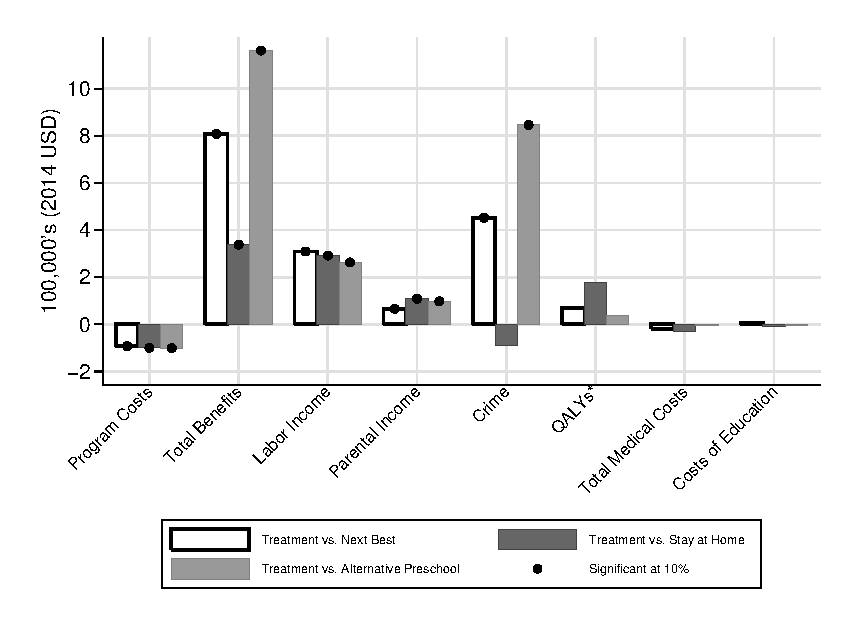
\includegraphics[width=\textwidth]{output/abccare_npvs2.eps}
\end{subfigure}%
\begin{subfigure}[h]{0.5\textwidth}
		\centering
		\caption{Females}
		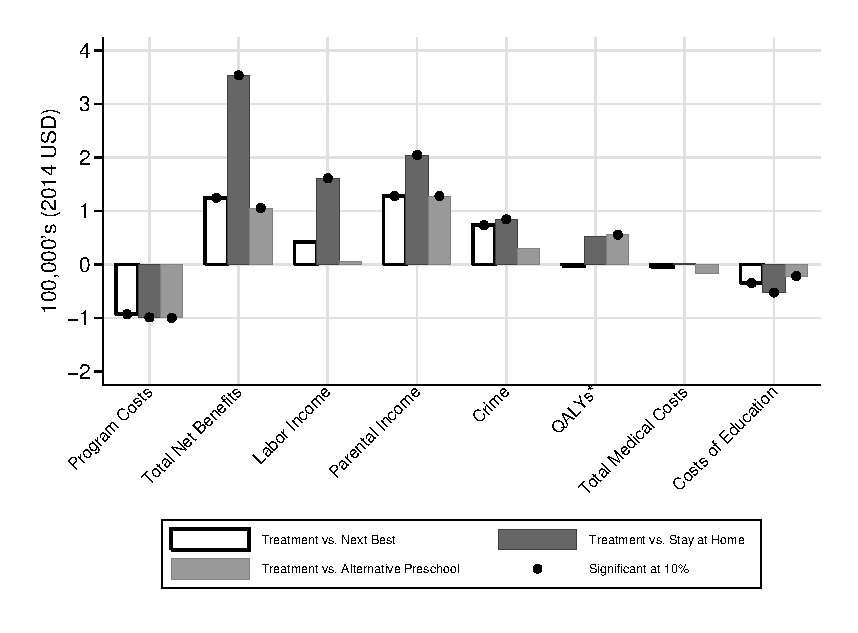
\includegraphics[width=\textwidth]{output/abccare_npvs1.eps}
\end{subfigure}
\footnotesize \justify
Note: This figure displays the life-cycle net present values of the main components of the cost/benefit analysis of ABC/CARE from birth to forecasted death, discounted to birth at a rate of 3\%. ``Treatment vs. Next Best'': compares the treatment to the control group. ``Treatment vs. Stay at Home'': compares the treatment group to those subjects who stayed at home. ``Treatment vs. Alternative Preschool'': compares the treatment group to those subjects who attended alternative preschools. The latter two are based on matching estimators that account for selection on observable variables. By ``net" we mean that each component represents the total value for the treatment group minus the total value for the control group. Program costs: the total cost of ABC/CARE, including the welfare cost of taxes to finance it. Total net benefits: are for \textit{all} of the components we consider. Labor income: total individual labor income from ages 20 to the retirement of program participants (assumed to be age 67). Parental labor income: total parental labor income of the parents of the participants from when the participants were ages 1.5 to 21. Crime: the total cost of crime (judicial and victimization costs). To simplify the display, the following components are not shown in the figure: (i) cost of alternative preschool paid by the parents of control group children; (ii) the social welfare costs of transfer income from the government; (iii) disability benefits and social security claims; (iv) costs of increased individual and maternal education (including special education and grade retention); (v) total medical public and private costs. Inference is based on non-parametric, one-sided $p$-values from the empirical bootstrap distribution. We indicate point estimates significant at the $10\%$ level.\\
*The treatment vs. stay at home net present value is sizable and negative (-\$123,498.2); its standard error is \$62,745.72.\\
**QALYs refers to the quality-adjusted life years. Any gain corresponds to better health conditions until forecasted death, with $\$150,000$ (2014 USD) as the base value for a year of life.
\end{sidewaysfigure}

\section{Understanding Recent Benefit-Cost Analyses} \label{section:bcaestimates}

We use our analysis to examine the empirical foundations of the approach to benefit/cost analysis taken in a prototypical study of \citet{Kline_Walters_2016_QJE}, which in turn is based on estimates taken from \citet{Chetty_Friedman_etal_2011_QJoE}. Although widely emulated, this approach offers an imprecise approximation of benefit/cost ratios with questionable validity. Examples of application of this approach include \citet{Attanasio_Kugler_Meghir_2011_AEJAE}, \cite{Behrman-et-al_2011_JHR-Progresa}, and \cite{Lafortune_etal_2018_Reform_AEJAE}.

\citet{Kline_Walters_2016_QJE} use data from the Head Start Impact Study (HSIS) and report a benefit/cost ratio between $1.50$ and $1.84$.\footnote{HSIS is a one-year-long randomized evaluation of Head Start.} Their analysis proceeds in three steps: (i) calculate program treatment effects on IQ measured around age 5;\footnote{They use an index based on the Peabody Picture Vocabulary and Woodcock Johnson III Tests.} (ii) monetize this gain using the return to the IQ measured between ages 5 and 7 in terms of net present value of labor income at age 27 using the estimates of \citet{Chetty_Friedman_etal_2011_QJoE};\footnote{The \citet{Chetty_Friedman_etal_2011_QJoE} return is based on Stanford Achievement Tests.}$^,$\footnote{For this comparison exercise, we interpret the earnings estimated in \citet{Chetty_Friedman_etal_2011_QJoE} to be equivalent to labor income.}$^,$\footnote{Calculations from \citet{Chetty_Friedman_etal_2011_QJoE} indicate that a 1 standard deviation gain in IQ at age 5 implies a $13.1\%$ increase in the net present value of labor income through age 27. This is based on combining information from Project Star and administrative data at age 27.} and (iii) calculate the benefit/cost ratio based on this gain and their own calculations of the program's cost.\footnote{Their calculation assigns the net present value of labor income through age 27 of $\$385,907.17$ to the control-group participants, as estimated by  \citet{Chetty_Friedman_etal_2011_QJoE}.}$^,$\footnote{All monetary values that we provide in this section are in 2014 USD. We discount the value provided by \citet{Chetty_Friedman_etal_2011_QJoE} to the age of birth of the children in our sample (first cohort).}

\begin{table}[!htbp]
\begin{threeparttable}
\caption{Alternative Cost/Benefit Analyses Calculations}
\label{table:comparing}
\centering
\footnotesize

\begin{tabular}{cllcc}
\toprule
Age & \mc{1}{c}{NPV Source} & Component & \citet{Kline_Walters_2016_QJE} & Authors' Method \\
& & & Method & \\
\midrule
\multirow{2}{*}{27} & \cite{Chetty_Friedman_etal_2011_QJoE} & Labor income & 0.58 (s.e. 0.28) &  \\
& ABC/CARE-calculated & Labor income & 0.09 (s.e. 0.04) &  1.09 (s.e. 0.04)\\
\midrule
\multirow{2}{*}{34} & ABC/CARE-calculated & Labor income & 0.37 (s.e. 0.04) & 0.15 (s.e. 0.05) \\
& ABC/CARE-calculated & All & 1.21 (s.e. 0.05) &  3.20 (s.e. 1.04) \\
\midrule
\multirow{2}{*}{Life-cycle} &  ABC/CARE-calculated & Labor income & 1.56 (s.e. 0.08) & 1.55 (s.e. 0.76) \\
& ABC/CARE-calculated & All & 3.80 (s.e. 0.29) & 7.33 (s.e. 1.84) \\
\bottomrule
\end{tabular}

\begin{tablenotes}
\footnotesize
\item Note: This table displays benefit/cost ratios based on the methodology in \citet{Kline_Walters_2016_QJE} and based on our own methodology. Age: age at which we stop calculating the net present value. NPV Source: source where we obtain the net present value. Component: item used to compute net present value (all refers to the net present value of all the components). \citet{Kline_Walters_2016_QJE} Method: estimate based on these authors' methodology. Authors' Method: estimates based on our methodology. Standard errors are based on the empirical bootstrap distribution.
\end{tablenotes}
\end{threeparttable}
\end{table}

To analyze how our estimates compare to those based on this method, we present a series of exercises in the fourth column of Table~\ref{table:comparing}. For purposes of comparison, the fifth column of Table~\ref{table:comparing} shows the analogous estimates based on our own samples and forecasts.

In the first exercise, we calculate the benefit/cost ratio using both the ``return to IQ'' and the net present value of labor income at age 27 reported in \citet{Chetty_Friedman_etal_2011_QJoE}. This calculation is the same type of calculation as that used in \citet{Kline_Walters_2016_QJE}. In the second exercise, we perform a similar exercise but use our own estimate of the net present value of labor income at age 27.\footnote{This allows us to compute our own ``return to IQ'' and impute it to the treatment-group individuals.} In this exercise, the standard errors account for variation in the return because we calculate the return in every bootstrapped re-sample. In that sense, our approach is a valid account of underlying uncertainties when compared to \citet{Kline_Walters_2016_QJE}, who do not account for estimation error in reporting standard errors. The return is smaller because our sample is much more disadvantaged than that of \citet{Chetty_Friedman_etal_2011_QJoE}.

The remaining exercises are similar, but we (i) increase the age range over which we calculate the net-present value of labor income; or (ii) consider the value of all the components we analyze throughout the paper, in addition to labor income. The more inclusive the benefits measured and the longer the horizon over which they are measured, the greater the benefit/cost ratio. The final reported estimate, 7.33, is our baseline estimate that incorporates all of the components across the life cycles of the subjects.

Our methodology provides a more accurate estimate of the net present value (and the return to IQ) of the program. We better quantify the effects of the experiment by considering benefits over the whole life cycle. We also better approximate the statistical uncertainty of our estimates by considering both the sampling error in the experimental and auxiliary samples and the forecast error due to the interpolation and extrapolation. Proceeding in this fashion enables us to examine the sensitivity of each of the components in our study.

\section{Summary and Contextualization of Results} \label{section:conclusion}

In this paper, we go beyond the analysis of batteries of short-term outcomes on test scores or analysis of isolated domains of human capital to evaluate the effectiveness of high-quality early childhood education. We exploit data generated by a high-quality early childhood education program with longitudinal follow up. The available follow-ups go from birth to when the program participants were in their mid 30s. Using economic models, we supplement the experimental data with non-experimental datasets to estimate life-cycle benefits and costs to evaluate the program's social efficiency.

Our analysis accounts for multiple sources of statistical and modeling uncertainty. We go beyond current analyses that only quantify a single, short-term treatment effects to forecast labor income without providing a sense of statistical and modeling uncertainty. We quantify long-term costs and benefits and provide a life-cycle analysis. We quantify and monetize health outcomes, a novel feature in the evaluation of early childhood programs.

We estimate that the internal rate of return (benefit/cost ratio) of the program ranges from 8.0\% to 18.3\% (1.52 to 17.40). These results indicate that investing in this program is highly socially profitable. ABC/CARE does not represent what is currently offered as early childhood education, although it has been widely replicated around the world. ABC/CARE is a prototype of what early childhood education should be.

A fundamental question for policy implementation is: Would these returns hold if the program is replicated elsewhere? On one hand, it is true that ABC/CARE was implemented in a specific and economically advantaged setting. On the other hand, the value of this paper is to provide the life-cycle benefits of this program, which essential elements could be replicated. Of course, its long term effectiveness needs to be complemented with the provision of schooling and job opportunities because economic opportunity complements the skills that this program fosters.
%References
\singlespace
\bibliographystyle{chicago}
\bibliography{heckman}

\end{document}
